\documentclass[openany,12pt]{report}

\setlength{\textwidth}{6.25in} % original 6.25

\setlength{\textheight}{8.9in}

\renewcommand{\baselinestretch}{1.3}

%\headheight 12.0pt

\oddsidemargin 20pt    %  Left margin on odd-numbered pages.

\evensidemargin 20pt   %  Note that \oddsidemargin = \evensidemargin

\topmargin 0pt

%\headsep 10pt

\footskip 10.0pt

\usepackage {graphics}

\usepackage[colorinlistoftodos]{todonotes}

\usepackage{comment}

%\usepackage {algorithm}

%\usepackage {algorithmic}
\usepackage{hyperref}
\usepackage{color}
\usepackage{lastpage} % for the number of the last page in the document
\usepackage{fancyheadings}
\pagestyle{fancy}
\usepackage {epsfig}
\usepackage {graphicx}
\usepackage{float}
\usepackage{array} % for making text bold in table
\usepackage{longtable}
%\usepackage[dvips, bookmarks, colorlinks=false]{hyperref}
%\usepackage{hyperref} %for creating links in the pdf version and other additional pdf attributes, no effect on the printed document

%*****************************Title Page**************************************************************

\begin{document} % Begin document "environment".
	\lhead{}
	\chead{}
	\rhead{Artificially Intelligent Traffic Management System}
	\lfoot{ MET's Institute of Engineering}
	\setlength{\headrulewidth}{0.4pt}
	\setlength{\footrulewidth}{0.4pt}
	\fontsize{12}{15}
	\begin{titlepage}
		\begin{center}
			%\vspace{0.2in}
			{\bf A Preliminary Report on} \\
			\vspace{0.3in}
			{\Large \bf ``Artificially Intelligent Traffic Management System''}\\
			\vspace{0.3in}
			SUBMITTED TO THE SAVITRIBAI PHULE PUNE UNIVERSITY, PUNE\\
			IN THE PARTIAL FULFILMENT OF THE REQUIREMENTS \\
			FOR THE AWARD OF THE DEGREE \\
			\vspace{0.2in}
			OF\\  
			\vspace{0.2in}
			BACHELOR OF ENGINEERING (COMPUTER ENGINEERING)\\
			(Academic Year: 2021-22)\\
			\vspace{0.2in}
			
			{\it SUBMITTED BY}\\
			
			\vspace{0.2in}
			
			{\bf Mr. Saquib Akhtar Aneesur Rahman}\hspace*{\fill}{\bf (Exam Seat No. B150474298)}\\
			{\bf Mr. Giwil Gidwani }\hspace*{\fill}{\bf (Exam Seat No. B150474245)}\\
			{\bf Mr. Vrushabh Dattatray Nikam     }\hspace*{\fill}{\bf (Exam Seat No. B150474278)}\\
			{\bf Mr. Rutuja Rajesh Shinde    }\hspace*{\fill}{\bf (Exam Seat No. B150474304)}\\
			
			\vspace{0.4in}
			
			{\it Under the guidance of}\\
			
			\vspace{0.1in}
			
			{\bf Mr. Ravindra Aher}\\
			\vspace{0.4in}
			
			
			{\small DEPARTMENT OF COMPUTER ENGINEERING}\\
			\begin{figure*}[h]
				\centerline{\psfig{figure=./metbkc.eps,width=4.1in,height=0.5in}}
				\label{atcres}
			\end{figure*}
			{\large MET's Institute of Engineering,}\\
			{\small Adgaon, Nashik-422003}\\
			SAVITRIBAI PHULE PUNE UNIVERSITY\\
			\vspace{0.2in}
			{\small May, 2022}
		\end{center}
	\end{titlepage}
	
	%*****************************Certificate*************************************************************
	\fontsize{14}{16}
	\thispagestyle{empty}
	\begin{center}
		\begin{figure*}[h]
			\centerline{\psfig{figure=./metbkc.eps,width=7.2in,height=1.2in}}
			\label{atcres}
		\end{figure*}
		\vspace{0.1in}
		{\it \Huge  \textbf{Certificate}}
		\vspace{0.2in}\\
		{\it This is to Certify that the project report entitles}\\
		\vspace{0.2in}
		{\Large \bf ``Artificially Intelligent Traffic Management System''}\\
		\vspace{0.2in}
	\fontsize{13}{15}	
		{\bf Mr. Saquib Akhtar Aneesur Rahman}\hspace*{\fill}{\bf (Exam Seat No. B150474298)}\\
		{\bf Mr. Giwil Gidwani}\hspace*{\fill}{\bf (Exam Seat No. B150474245)}\\
		{\bf Mr. Vrushabh Dattatray Nikam}\hspace*{\fill}{\bf (Exam Seat No. B150474278)}\\
		{\bf Mr. Rutuja Rajesh Shinde}\hspace*{\fill}{\bf (Exam Seat No. B150474304)}\\
		
	\end{center}
	\fontsize{14}{16}
	\vspace{0.3in}
	{\it are bonafide students of this institute and the work has been carried out by them under
		the guidance of Mr. Ravindra Aher and it is approved for the partial fulfillment of the
		requirement of Savitribai Phule Pune University for the award of the degree of Bachelor
		of Engineering (Computer Engineering).}\\
	\vspace{0.2in}
	\vspace{0.7in}
	\noindent
	
	\hspace{0.1in} Project Guide  \hspace{1.5in}H.O.D \hspace{01.5in} Principal  \\
	\hspace{0.8in} (Mr. Ravindra Aher) \hspace{0.85in}(Dr. M. U. Kharat)\hspace{0.9in}(Dr. V. P. Wani)\\
	\vspace{0.2in}
	
	\begin{flushleft}
	{Place: Nashik}\\	
	{Date: \hspace{0.2 in}/\hspace{0.3 in}/}   \\
	\end{flushleft}		
	\newpage \pagenumbering{roman}
	%\vskip
	\chapter*{Acknowledgements}
	
	\hspace*{0.5 in}We have taken efforts in this project. However, it would not have been possible without the kind support and help of many individual and organizations. We would like to extend our sincere thanks to all of them. It gives us proud privilege to complete the project on \textbf{ ``Artificially Intelligent Traffic Management System''}. We are highly indebted to our internal guide \textbf{Mr. Ravindra Aher} for his guidance and constant supervision as well as for providing necessary information regarding the project and also for his support in completing the project.\\
	
	\hspace*{0.5 in}We are also extremely grateful to our respected H.O.D. (Computer Department) \textbf{Dr. M. U. Kharat} and \textbf{Dr. Priti Metange} (Project Co-ordinator) for providing all facilities and every help for smooth progress of project work.\\
	\\
	\hspace*{3.5 in}Mr. Saquib Akhtar Aneesur Rahman\\
	\hspace*{3.5 in}Mr. Giwil Gidwani \\
	\hspace*{3.5 in}Mr. Vrushabh Dattatray Nikam\\
	\hspace*{3.5 in}Ms. Rutuja Rajesh Shinde
	
	%*****************************Abstract*************************************************************
	\chapter*{Abstract\markboth{Abstract}{Abstract}}
	\hspace*{0.5 in}Congestion of traffic in urban areas and smart cities is one of the major issues with increasing population in metropolitan areas. Traffic jams are not only a cause of delay and inconvenience in day to day life but also a major source of noise and air pollution.
	Modern approaches to deal with this issue range from complicated software handling dozens of traffic signals throughout an entire city to simpler single-intersection solutions. However these can be costly, difficult to implement and may require a lot of manual monitoring.\\
	\\
	\hspace*{0.5in}This project proposes a traffic management system which uses concepts from artificial intelligence and graph theory to control and optimize traffic flow. Its aim is to optimize traffic flow on a small to medium scale in a manner which adapts to the real time changes in traffic.\\
	
	\newpage
	\tableofcontents
	\listoffigures
	\listoftables
	\newpage	
	\pagenumbering{arabic}
	
	
	
	
	%*****************************Chapter1 *****************************
	
	\chapter{Introduction}
	\hspace*{0.5in}This chapter briefly explains the need for an adaptive traffic management system and an overview of the implementation.\\
	
	\section{Overview}
	\hspace*{0.5in}Traffic congestion is becoming one of the critical issues in cities with increasing population and number of vehicles. They not only cause problems like delays and stress to drivers but also cause secondary problems like increasing fuel consumption, transportation costs and pollution.
	
	The causes of congestion can be divided into two categories, recurring and non recurring congestion. Recurring congestion can be expected to occur at the same time every weekday as a result of high volumes of commuter traffic traveling on roadways that are at or near their carrying capacity. Non-recurring congestion occurs as a result of an unexpected or non-typical event. Some causes of non-recurring congestion include: vehicular crashes, vehicle breakdowns, roadway construction, inclimate weather, and additional traffic resulting from special events. While non-recurring congestion can be unpredictable and difficult to treat, recurring congestion can be reduced by increasing road capacity or with the help of adaptive traffic control systems.
	
	There are several existing standardized solutions for adaptive traffic control such as SCOOT\cite{paper5}, SCAT\cite{paper6}, etc. which have been implemented in many major metropolitan cities. However, most suburban and urban areas use conventional traffic control systems such as manual traffic control or non adaptive automated traffic control. Manual control consists of an on-site traffic official guiding vehicles. Non adaptive automated traffic control refers to the use of fixed timers in traffic signals. Wide implementation of standardized adaptive traffic control is not possible due to lack of feasibility since it requires manual labor and installation of new sensors. Therefore a more feasible solution which reuses existing infrastructure is required.
	
	This project proposes an Artificially Intelligent Traffic Management System which uses existing CCTV feed and API data if needed to optimize traffic control over small to medium scale road networks. It uses an artificially intelligent agent or model to handle the complexity of day to day traffic in real-time. Furthermore, simulations will be performed to demonstrate and test the model.\\
	
	\section{Summary}
	\hspace*{0.5in}This chapter discusses the need for an intelligent traffic management system and also discussed a brief overview of the project.\\
	%*************************Chapter 2************************
	\chapter{Literature Survey}
	
	\hspace*{0.5in}This chapter consists of the various studies and research conducted on key concepts which are essential to create and understand the proposed system.
	
	\section{You Only Look Once: Unified, Real-Time Object Detection, Joseph Redmon, et al. \cite{paper1}}
	\hspace*{0.5in}Object detection comprises locating specific types of objects in an image or video. The output of a typical object detection algorithm consists of bounding box coordinates and a label of the object. YOLO (You Only Look Once) model consists of an extremely fast unified architecture for object detection. It makes use of a single neural network for predicting bounding boxes and class probabilities from a full image in a single evaluation. Hence, making it ideal for object detection in real time applications.\\
	
	\section{Traffic Congestion Detection from Camera Images using Deep Convolution Neural Networks, Pranamesh Chakraborty, et al. \cite{paper2}}
	\hspace*{0.5in}Recent improvements in computer vision algorithms have led to closed-circuit television (CCTV) cameras emerging as an important data source for determining the state of traffic congestion. To detect congestion in a traffic CCTV footage YOLO, a state-of-the-art real-time object detection algorithm is used. In the above mentioned paper, several object detection techniques were tested for congestion detection out of which YOLO showed the most promising results.\\
	
	\section{Smart Control of Traffic Light Using Artificial Intelligence, Mihir M. Gandhi, et al. \cite{paper3}}
	\hspace*{0.5in}Traffic signal timing plays an important role in controlling flow and efficiency of traffic.
	The above system makes use of vehicle count obtained from CCTV footage and uses it to  optimize green signal timing for each lane to optimize traffic flow at a single intersection. The aim of the project is to create a similar system and extend the scope of optimization to multiple adjacent intersections.\\
	
	\section{Comparison of Current Practical Adaptive Traffic Control Systems, Hongyun Chen, et al. \cite{paper4}}
	\hspace*{0.5in}Existing Adaptive Traffic Control Systems (ATCS) such as SCOOT, SCAT, OPAC, RHODES, etc. are being adapted by major cities in developed and developing countries. They can cover up to hundreds (OPAC) to even thousands (SCOOT, SCAT) of intersections. However, their implementation includes installation of additional sensors and can lead to very heavy costs which isn't feasible for smaller cities. Additionally, these systems do not take into consideration challenges such as power failure, non lane following traffic and mixed traffic which are common in Indian roads.\\
	\hspace*{0.5in}The aforementioned systems provide key algorithmic insights for developing a more feasible ATCS model. Furthermore, usage of existing inputs such as CCTV needs to be emphasized over installation of new sensors in order to help reduce costs.\\
	
	\section{Comparison of PPO and SAC Algorithms Towards Decision Making Strategies for Collision Avoidance Among Multiple Autonomous Vehicles, Abu Jafar Md Muzahid, et al.\cite{paper7}}
	\hspace*{0.5 in}Commonly used reinforcement learning algorithms, namely  PPO (Proximal Policy Optimization) and SAC (Soft Actor-Critic) were trained, evaluated and compared using Unity3D and ML-Agents.
	
	\section{A Deep Reinforcement Learning Approach for Traffic Signal Control Optimization, Zhenning Li, et al. \cite{paper8}}
	\hspace*{0.5 in} This paper demonstrates optimization of traffic signal control using reinforcement learning. Training a deep neural network using reinforcement learning can help improve adaptability od the signal.
	
	\section{Summary}
	\hspace*{0.5in}This chapter reviews research done on key concepts such as object detection and implementation of artificial intelligence with traffic signals which are essential to the proposed system. Existing solutions, their inner workings as well as their advantages and disadvantages were studied.\\
	
	
	%*************************Chapter 3 ************************
	
	\chapter{Problem Definition}
	
	\hspace*{0.5in}This chapter discusses the drawbacks of current systems implemented in suburban and urban areas and also defines the need and overall scope of an artificially intelligent traffic management system.\\
	
	\section{Need For Artificially Intelligent Traffic Management Systems}
	\hspace*{0.5in}Traffic congestion is becoming a critical issue with increasing population and automobiles in cities. The conventional systems which were suitable at the time of their installation may not be suitable in the present time due to the rising number of vehicles. Furthermore, upgrading these systems to the standards used in major metropolitan cities is often not feasible due to several factors such as manual labor and installation of new sensors. Owing to these factors, the majority of intersections make use of either manual control which includes traffic police officials guiding vehicles or non adaptive automatic control, which includes the use of fixed timers. In most scenarios these solutions may not be at par with the unpredictable rate of traffic flow. Hence, an intelligent, adaptive and feasible solution is needed.\\
	
	\section{Additional Features}
	\hspace*{0.5in}Additionally, the following points were kept in mind while developing and optimizing an automated traffic controlling system:\\
	
	\begin{itemize}
		\item{Ensuring signal times are between a maximum and minimum limit to avoid starvation.}
		\item{Indian traffic is not lane following and has a high amount of mixed traffic. System must be able to withstand these challenges.}
		\item{The system will be able to use the existing sensors and avoid installation of newer sensors in order to maintain feasibility.}
		\item{The system will be scalable within budget and able to handle an increasing number of vehicles.}
		%\item{Additional features such as incident detection, report generation and assistance for emergency or VIP vehicles can be added.}
	\end{itemize}
	
	
	
	\section{Summary}
	\hspace*{0.5in}This chapter discusses the need of artificially intelligent traffic management systems and the various points which must be kept in mind while developing said system.\\
	
	%*****************************Chapter 4******************
	
	\chapter{Analysis}
	\begin{comment}
		\hspace*{0.5in}This chapter describes the project plan adopted and determines the requirement analysis. We have implemented the project on the basis of Rapid Application Development (RAD) model and Model View Controller (MVC) model. The stake holders who participated in the requirement analysis process were the developers of Cognifront who will be among the end users of the Artificially Intelligent Traffic Management System for building M- Applications.
	\end{comment}
	
	\hspace*{0.5 in}This chapter describes the project plan adopted and determines the requirement analysis. The project was implemented on the basis of Agile model.\\
	\subsection{Agile Methodology and Version Control}
	
	\hspace*{0.5 in}Agile practices include requirements discovery and solutions improvement through the collaborative effort of self-organizing and cross-functional teams with their customer/end users ,adaptive planning, evolutionary development, early delivery, continual improvement, and flexible responses to changes in requirements, capacity, and understanding of the problems to be solved.\\
	\hspace*{0.5in}Agile methodology was implemented using scrum board and sprint planning on Jira by Atlassian.\\
	\hspace*{0.5in}Git is a free and open source distributed version control system designed to handle everything from small to very large projects with speed and efficiency.\\
	\hspace*{0.5in}Git version control was implemented using GitHub.
	\begin{figure}[H]
			\centering
			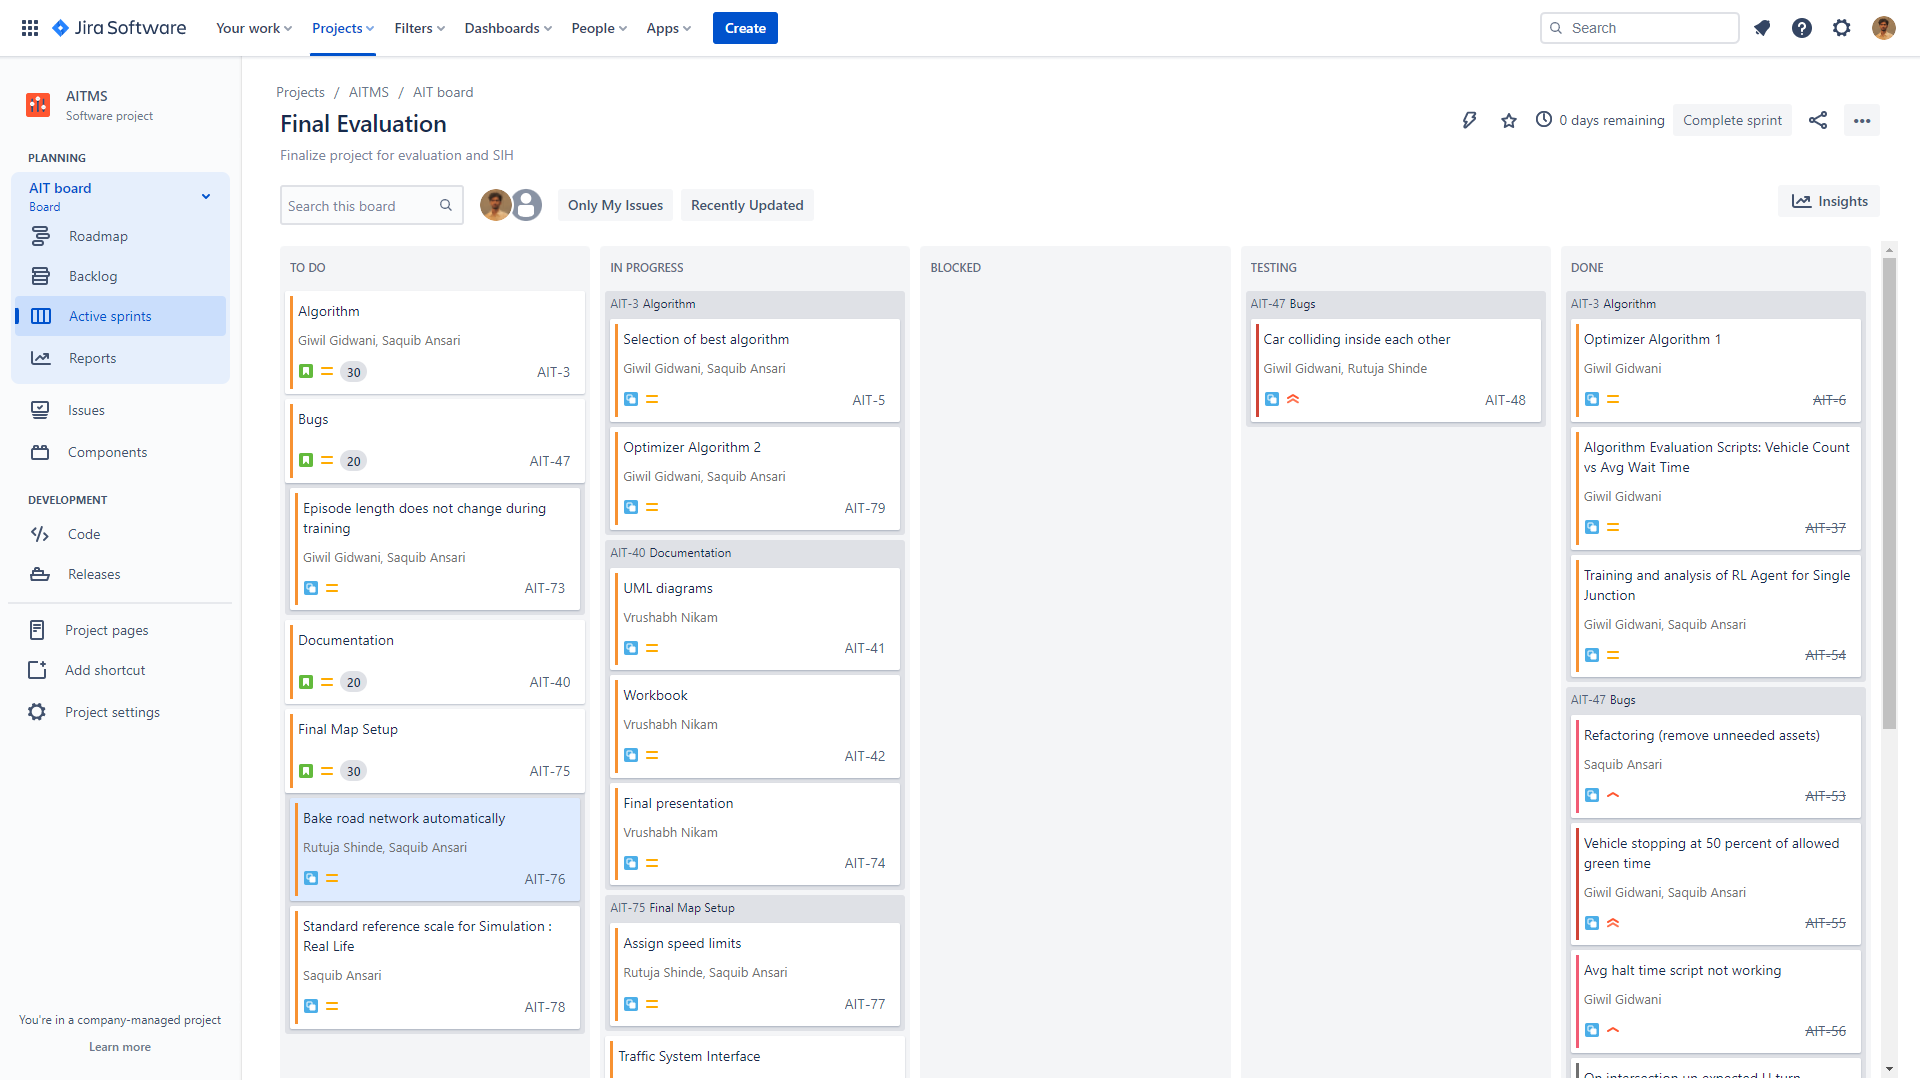
\includegraphics[width=6in]{./Diagrams/PNG/jira}
			\caption{AITMS Jira Board}
	\end{figure}	
	
	\begin{figure}[H]
			\centering
			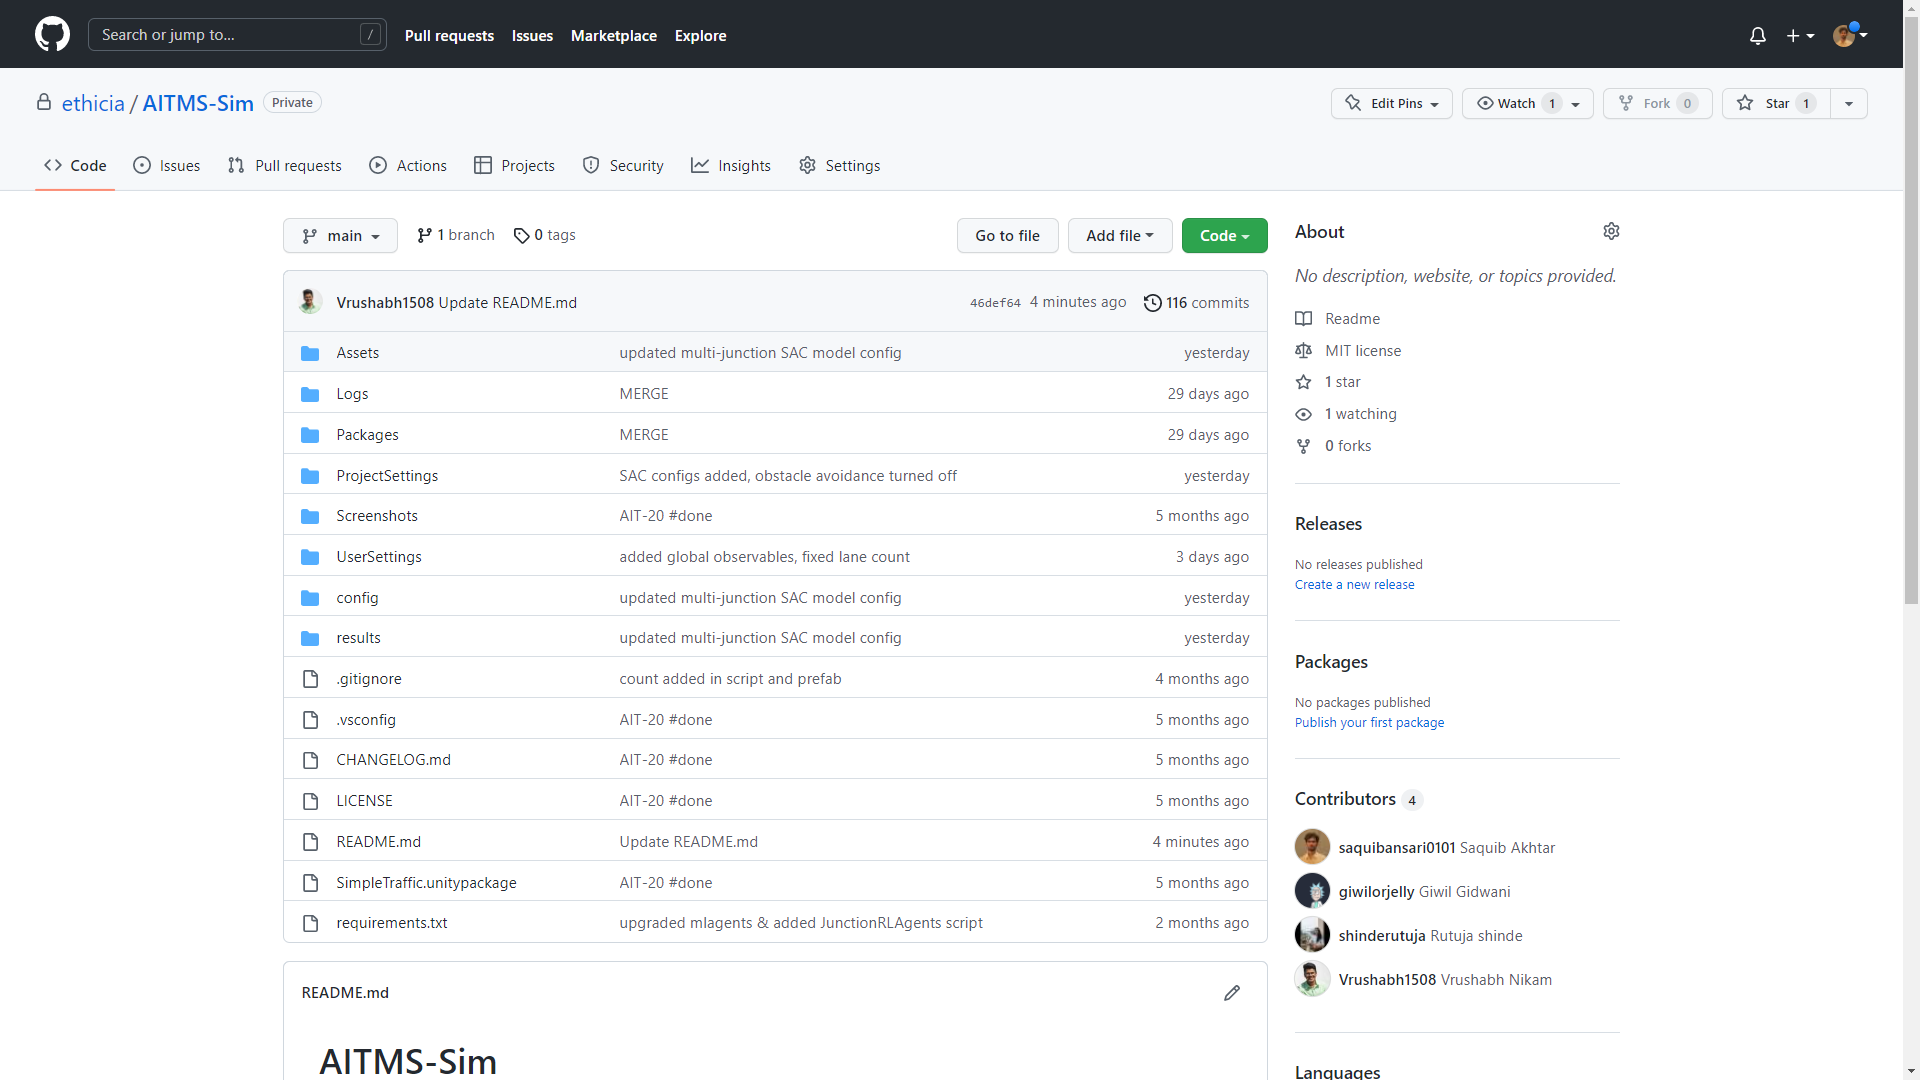
\includegraphics[width=6in]{./Diagrams/PNG/github}
			\caption{AITMS GitHub Repository}
	\end{figure}	
	
	\section{Project Plan}
	
	\subsection{Project Plan for Semester I}
	
	\hspace*{0.5 in}The following Table 4.1 describes the project plan for semester I. It describes the various activities and accountability of the developers for the respective modules. Following are the major activities carried out in this plan :
	\begin{itemize}
		\item{Identifying the functional requirements.}
		\item{Designing of the Framework.}
		\item{Studying the necessary development tools and technologies.}
	\end{itemize}

	\begin{table} [htb]
		\centering
		\begin{tabular}{| p{1.2 cm}| p{5 cm}| p{2.5 cm}| p{2.5 cm}| p{3 cm}| }\hline
			\textbf{Phase}	&\textbf{Activity}	&\textbf{Start Date}	&\textbf{End Date} &\textbf{Group Members}\\\hline\hline
			1 &
			Selection of Project Topic	&
			06-09-2021 	&
			13-09-2021 &
			Team \\\hline

			1 &
			Analysis of Smart Traffic Management System and Identification of System Requirements &
			19-09-2021 &
			03-10-2021 &
			Team\\\hline

			1 &
			Study of Implemented Solutions &
			11-10-2021 &
			21-10-2021 & 
			Saquib, Giwil\\\hline
			1 &
			UML Diagram Design &
			23-10-2021 &
			06-11-2021 &
			Vrushabh,Rutuja \\\hline
			
			1 &
			Presentation &
			06-11-2021 &
			08-11-2021 &
			Team \\\hline
			
			1 &
			Simulation Framework Design &
			20-11-2021 &
			28-11-2021 &
			Team \\\hline

			1 &
			Design Prototype of Navigation Sections &
			6-12-2021 &
			10-12-2021 &
			Team\\\hline
			
		\end{tabular}
		\caption{Planner and Progress Report I for AITMS}
		\label{tab:nnwork}
	\end{table}
	\newpage
	\subsection{Summary for Semester I}
	\hspace*{0.5 in}This chapter describes the implementation details of the project plan for
Semester I. It briefly discusses functional requirement specification, design prototype, and project 
problem statement of AITMS.


	\subsection{Project Plan for Semester II}
	
		\hspace*{0.5 in}The following Table 4.2 describes the project plan for semester II. It describes the various activities and accountability of the developers for the respective modules. Following are the major activities carried out in this plan :
		\begin{itemize}
			\item{Define Programming Standards.}
			\item{Development of project in 3 Milestones.}
			\item{Formal Technical Review and Testing.}
		\end{itemize}
	
		\begin{table} [htb]
			%\centering
			\begin{tabular}{| p{1.2 cm}| p{5 cm}| p{2.5 cm}| p{2.5 cm}| p{3 cm}| }\hline
				\textbf{Phase}	&\textbf{Activity}	&\textbf{Start Date}	&\textbf{End Date} &\textbf{Group Members}\\\hline\hline

				2 
				&Development of Traffic Components
				&01-01-2022 	
				&20-02-2022 &Team \\\hline

				2 
				&Development of RL Agents Module
				&26-02-2022 
				&15-03-2022 &Team\\\hline

				2 
				&Experimenting Various Reward Mechanisms
				&17-03-2022 
				&15-04-2022 &Team\\\hline

				2 
				&Training and Evaluating Optimized Models
				&20-04-2022 
				&30-04-2022 & Team \\\hline

				2 
				&Formal Technical Review 
				&04-05-2022 
				&06-05-2022 &Team \\\hline

				2 
				&Testing and Bug Fixing  
				&09-05-2022 
				&12-05-2022 &Team\\\hline
				
			\end{tabular}
			\caption{Planner and Progress Report II for AITMS}
			\label{tab:nnwork}
		\end{table}
	
	
	\newpage
	\subsection{Summary for Semester II}
	\hspace*{0.5 in}This chapter explains implementation details of the project plan for
Semester II. Necessary functions and the desirable functions of AITMS are briefly discussed.
	
	\section{Requirement Analysis}
	
	\subsection{Necessary Functions}
	\begin{itemize}
		\item{\textbf{Simulation: }Simulation provides creation of road maps for traffic system, it helps in simulating real-time traffic and visualizing traffic densities. It consists of a wide variety of traffic component presets which make creation of road maps easier through drag and drop. It is implemented in Unity3D.}
		\item{\textbf{RL Agents Scripts: }It consists of a set of scripts which help define training parameters and reward mechanisms for MLAgents. It is developed keeping reusability in mind, in order to allow the users to program and experiment with different reward mechanisms.}
		\item{\textbf{Training Smart Traffic Signals: }The primary purpose of the system is to provide a platform for training smart traffic signals using reinforcement learning. The trained models are able to reduce waiting time by providing optimal green signal time as output such that maximum waiting vehicles are able to pass through without stalling other phases for longer than necessary.}
	\end{itemize}
	
	\subsection{Desirable  Functions}
	\begin{itemize}
		%\item{Assistance to emergency and VIP vehicles.}	
		%\item{Traffic incident detection.}
		%\item{Real-time Traffic Congestion Detection.}
		%\item{Real-time Statistics.}
		\item{\textbf{Real-time Traffic Congestion Detection: }Having access to CCTV footage as well as vehicle counts for all the phases in real-time make it possible to detect congestion in real-time.}
		\item{\textbf{Real-time Statistics: }Collection of essential parameters such as vehicle counts and phase time provide scope for generating statistical reports on traffic flow in real-time.}
	\end{itemize}
		
	\section{Summary}
	\hspace*{0.5in}This chapter describes the implementation details of the project plan for Semester I and Semester II. The necessary functions and the desirable functions of Artificially Intelligent Traffic Management System were also studied.
	%*****************************Chapter5***************
	\chapter{Design}
	\hspace*{0.5in}This chapter describes the Software Requirement Specification (SRS) to be implemented for Artificially Intelligent Traffic Management System. It also explains the architecture of the system and external interface requirements.\\
	
	\section{Software Requirement Specifications}
	\hspace*{0.5in} The Software Requirement Specification describes the scope of the project, operating environment, user characteristics, design and constraints. It also elaborates the system architecture of the Artificially Intelligent Traffic Management System.
	
	\subsection{Project Scope}
	
	\hspace*{0.5in}The main purpose of developing the Artificially Intelligent Traffic Management System is for the welfare of the public and to reduce the pollution caused by traffic congestion. The issue of transportation is one of the most problematic issues in the country, and in the world at large. In an age where a person has a private car, and especially in countries where there is a failing public transport system, traffic jams and the countless accidents that accompany road congestion harm the economic, political and social aspects in both the public and private sectors. the transportation systems used by transportation agencies around the world are not adapted to modern transportation - these are systems designed decades ago, when the amount of cars on the roads was much smaller than today, and the transportation nodes were relatively simple. today, innovative technologies for computerized transportation management are in use, but these turned out to be extremely expensive, and due to budget shortages and even many cuts in the transportation budget, transportation agencies are often forced to give up these systems and stick with the old systems. Countries such as Australia, Singapore, and a number of U.S. states have adopted transportation management technologies on a massive scale (for example, GLIDE, SCATS\cite{paper6} - these are huge economic investments, these are proving themselves as highly prudent and effective investments. The purpose of the software is to enable the optimization of traffic signals through implementation of machine learning on data collected at traffic signals, making them more adaptive to real time changes in traffic flow. The software is made to be intuitive and accessible as much as possible, while maintaining accuracy, maximum detail, level of performance And high efficiency.
	\\The scope of Artificially Intelligent Traffic Management System can be considered as a collection of reusable piece of code, 3D roadway components, trained models and include files that can be used by the developer for developing more advanced systems and also considering the following points :
	\begin{itemize}
		\item{Warehousing of parametric data and reports to analyze periodic patterns and improve optimization using it (data science)}
		\item{Making AITMS compatible with each other so that neighboring solutions can work together providing another layer of optimization with added scalability}
		\item{Providing a platform for simulating roadmaps and training smart signals; allowing the user maximum flexibility in design of maps and smart signal models}
	\end{itemize}
	
	\subsection{Operating Environment}
	\hspace*{0.5in}The proposed system will require an operating environment with appropriate version of Windows or Linux OS, Python, Unity3D and sufficient computation power through GPUs.
	
	\subsection{Design and Implementation Constraints}
	\hspace*{0.5in}The key restriction here will be to verify the validity of the report, which is not always feasible.Security threats may be involved.\\
	\begin{itemize}
		\item{\textbf{Memory:} Minimum 16GB RAM}
		\item{\textbf{CPU:} Intel Core i5 - 8300H or equivalent\textbackslash higher.}
		\item{\textbf{GPU:} Nvidia GTX 1050ti or equivalent\textbackslash higher.}
		\item{\textbf{LAN for CCTV:}  CCTV feed from intersections to the server room.}
		\item{\textbf{Operating System:}  This application works on Windows and Linux.}
	\end{itemize}
	
	\subsection{Assumptions}
	\hspace*{0.5in}AITMS functions based on the following assumptions.
	\begin{itemize}
		\item{Inputs such as vehicle count, phase intervals and current phase are obtainable from the junction in real time.}
		\item{It is possible to interface traffic signals with AITMS in a way which allows AITMS to set phase intervals and traffic signal state for each lane.}
		\item{The Admin has a
			computer with graphic card, gets to monitor intersections and rest of the system is automated.}
	\end{itemize}

	\subsection{Dependencies}
	\hspace*{0.5in}AITMS requires the following software dependencies to be fulfilled for proper functioning.
	\begin{itemize}
		\item{\textbf{Python v3.7.13}\\
			Python is a high-level, interpreted, general-purpose programming language. Its design philosophy emphasizes code readability with the use of significant indentation. Python is dynamically-typed and garbage-collected. }
		\item{\textbf{Unity3D v2020.3.32f}\\
			Unity is a game development platform. Unity is used to build high-quality 3D and 2D games and simulations, deploy them across mobile, desktop, VR/AR, consoles or the Web, and connect with loyal and enthusiastic players and customers.}\\
		\item{\textbf{Unity ML-Agents v1.0.8}\\
			The Unity Machine Learning Agents Toolkit (ML-Agents) is an open-source project that enables games and simulations to serve as environments for training intelligent agents using deep reinforcement learning and imitation learning.}
		\item{\textbf{PyTorch v1.8.1}\\
			PyTorch is an open source machine learning framework based on the Torch library, used for applications such as computer vision and natural language processing, primarily developed by Facebook's AI Research lab. It is free and open-source software released under the Modified BSD license.}
		
	\end{itemize}
	
	
	\newpage
	\section{System Architecture}
	
	\hspace*{0.5in}The overall architecture can be viewed in the figure 5.1 in the form of a  3 layer architecture consisting of physical intersection, intersection node and the optimizer.\\
	\begin{figure}[H]
		\centering
		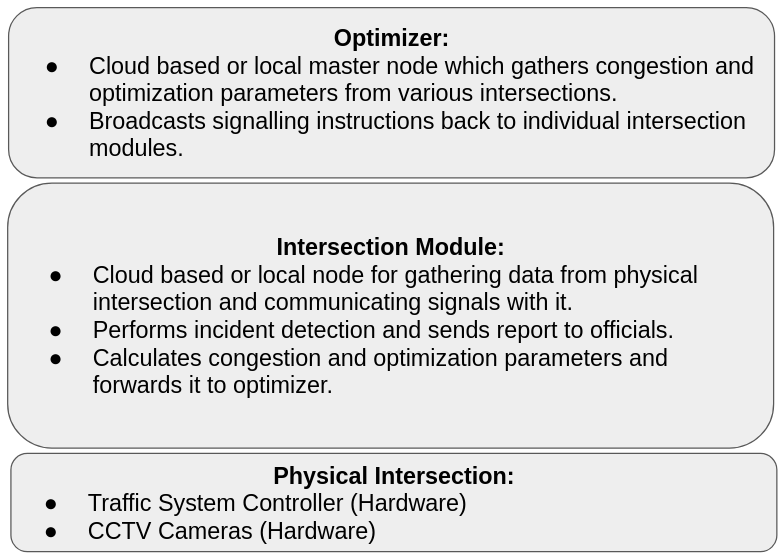
\includegraphics[width=5.2in,height=4.5in]{./Diagrams/PNG/layered_architecture}
		\caption{Layered form of System Architecture}
	\end{figure}
	
	\hspace*{0.5in}The lowermost layer i.e. the physical intersection consists of the physical traffic signal controllers and CCTV cameras. This layer contains the pre-existing infrastructure used for controlling traffic. The traffic signal controller must provide an interface to obtain and control its state. Furthermore, real-time CCTV footage must be made available to the model.\\
	
	\hspace*{0.5in}The intermediate layer consists of intersection nodes (software). Each intersection node represents a single traffic intersection. Intersection nodes serve the following primary functions:\\
	
	\begin{itemize}
		\item{Collecting CCTV footage and other data from physical intersection layer and APIs (if required by optimizer).}
		\item{Obtaining optimizer parameters from the collected raw data. For example, obtaining vehicle count from CCTV footage using YOLO. The intersection node then forwards this data to the optimizer.}
		\item{Intersection nodes also receive timing signals as outputs from the optimizer, their task is to then interface these signals onto the controller.}
	\end{itemize}
	
	\hspace*{0.5in}Aside from the above functions, the intersection nodes can also be used to perform extra tasks such as incident detection and sending reports on traffic incidents and congestion to traffic officials. It must be noted that since intersection nodes are services in execution, they can be executed over cloud or locally depending on feasibility. Depending on availability of computation power and hardware setup, a single computing device can hold multiple intersection nodes as well.\\
	
	\hspace*{0.5in}The uppermost layer consists of the optimizer. The optimizer is the master node which receives the required data from all the intersection nodes and executes the optimization algorithm. The optimization algorithm gives the signal timing details as output in terms of green signal time which is broadcasted back to the respective intersection nodes.\\
	
	\hspace*{0.5in}Several optimization algorithms were selected which can be applied depending on their performances on a simulation consisting of a specific map. It should also be noted that different optimization algorithms may be suited for different maps.\\
	\hspace*{0.5in}The following figure 5.2 illustrates the system architecture for 3 intersections.
	
	\begin{figure}[H]
		\centering
		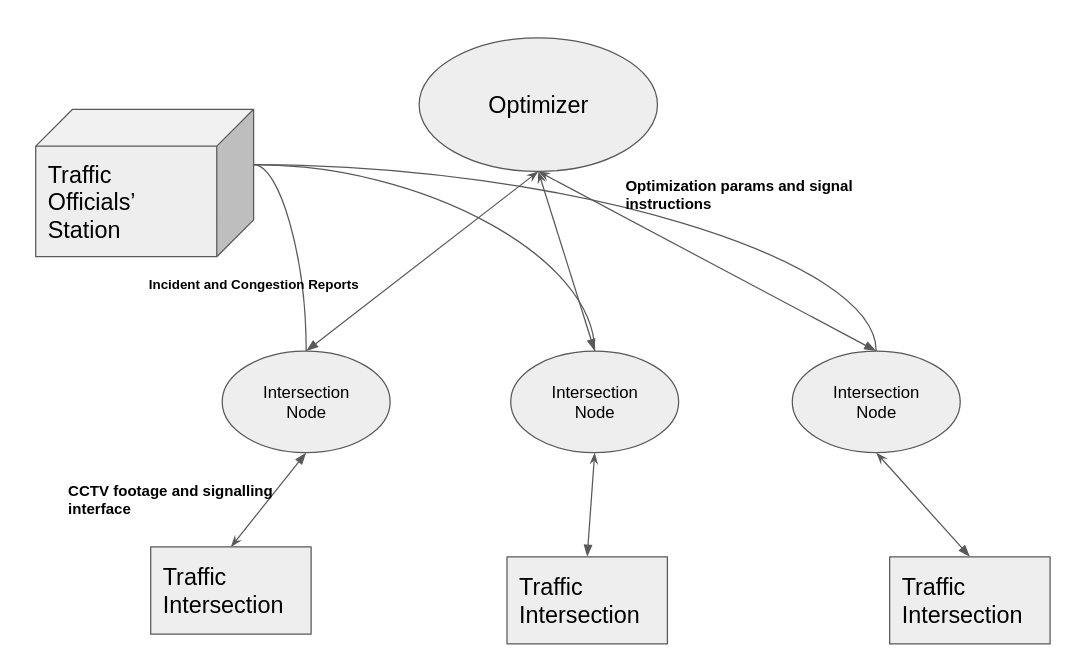
\includegraphics[width=6.5in,height=5.5in]{./Diagrams/PNG/architecture}
		\caption{System Architecture Illustration}
	\end{figure}
	
	\begin{comment}
		content...
		
		\section{External Interface Requirement}
		
		\subsection{User Interfaces}
		
		\begin{itemize}
			\item{\textbf{Desktop Application:}  Using the desktop application the end user will be able to provide the M-Learning content for the application to be developed using the Artificially Intelligent Traffic Management System.}
			\item{\textbf{M-Learning Application:}  The M-Learning application will provide a Graphical User Interface which will consist of several screens which the end user will be able to navigate to consume learning.}
		\end{itemize}
		
		\subsection{Hardware Interfaces}
		\begin{itemize}
			\item{\textbf{Mobile Devices:} The M-Learning applications built using the framewok will be deployed on mobile devices like smart-phones and tablets supporting Android operating system version 2.2 and above.}
			\item{\textbf{SD card:}  The M-Learning application will load the learning content stored on the SD card. End user will be able to write on the SD card as well.}
		\end{itemize}
		
		\subsection{Communication Interfaces}
		\hspace*{0.5in}The M-Learning application will be communicating through the internet via a Transmission Control Protocol of the TCP/IP suite for Social Networking Interface(SNI) and video streaming.
		
	\end{comment}
	\section{Software System Attribute}
	\begin{itemize}
		
		\item{\textbf{Reliability:} The traffic management system should be reliable with necessary fallbacks in case of technical failuers.}
		
		\item{\textbf{Maintainability:}  The Artificially Intelligent Traffic Management System shall be well documented and easy for developers to improve on}
		
	\end{itemize}
	
	\section{Data Flow Diagram}
	
	\hspace*{0.5in}The Data Flow Diagram explains the flow of information in the project, i.e. it indicates from where data or information is received (input) and to where it is sent (output). The Data Flow Diagrams for the project are given idn figure 5.3 and figure 5.4:\\
	
	\begin{figure}[H]
		\centering
		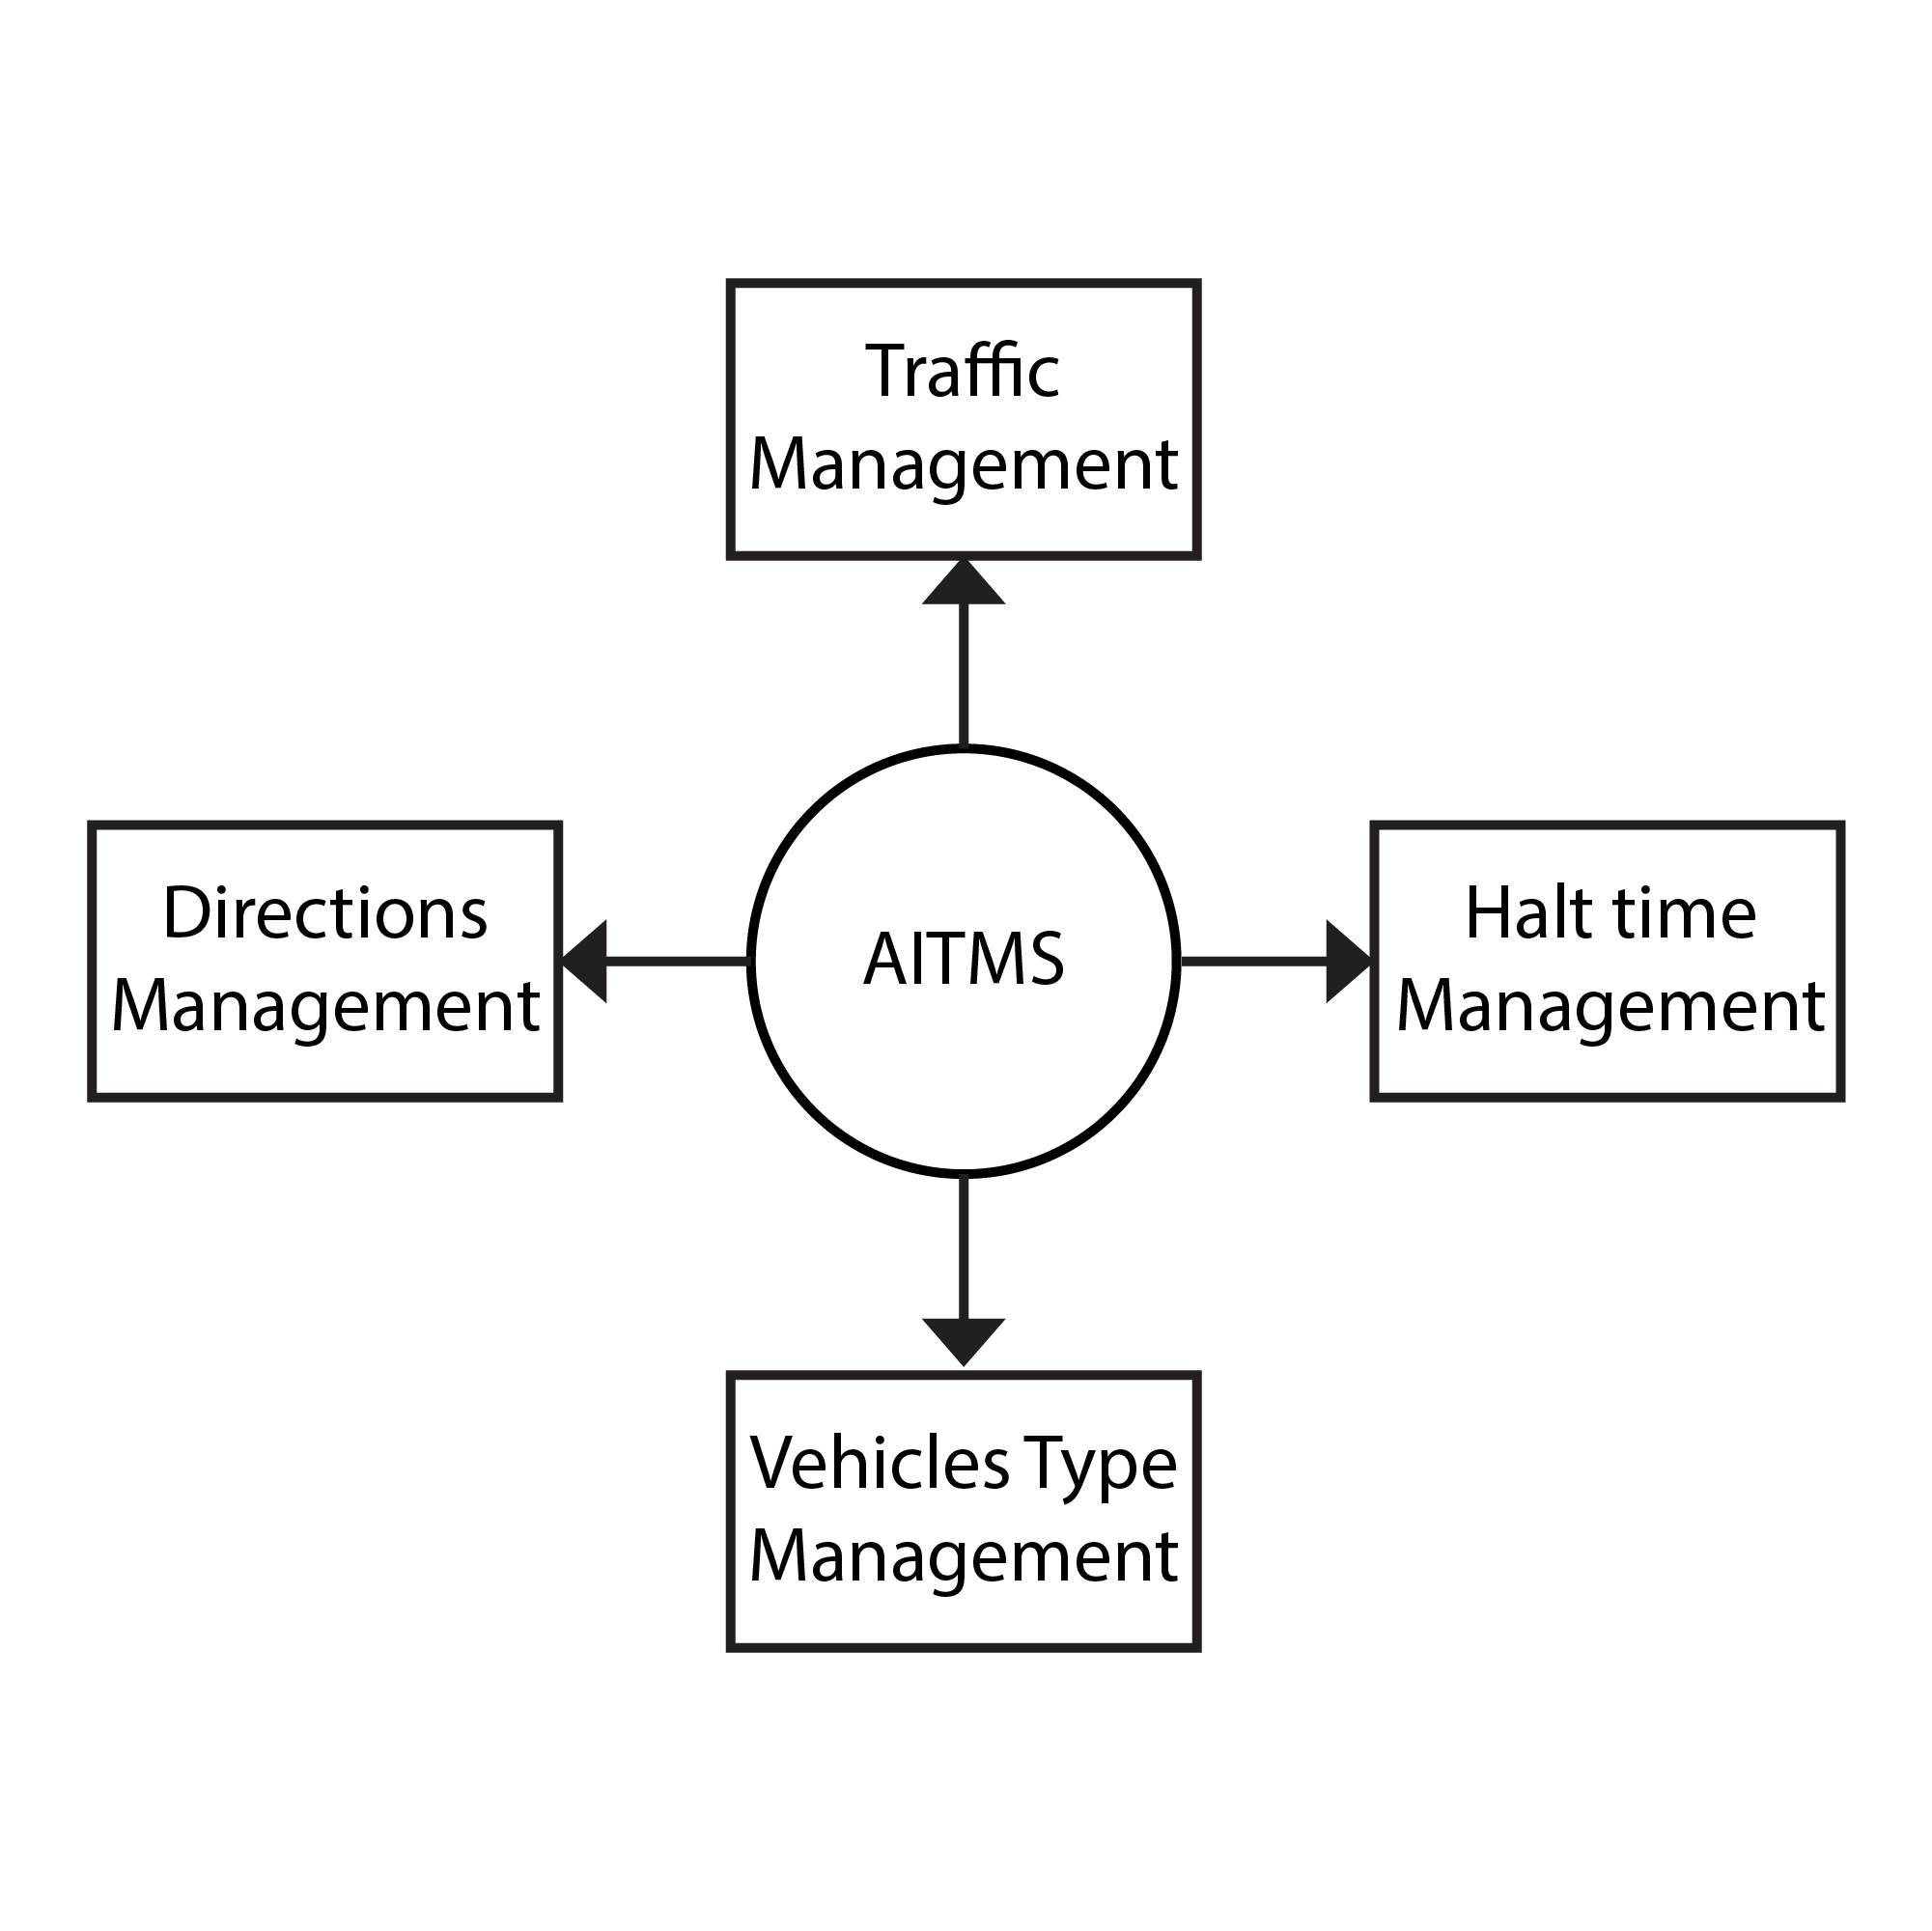
\includegraphics[height=3.3in]{./Diagrams/PNG/dataflow}
		\caption{Level 0 Data Flow Diagram}
	\end{figure}
	
	\begin{figure}[H]
		\centering
		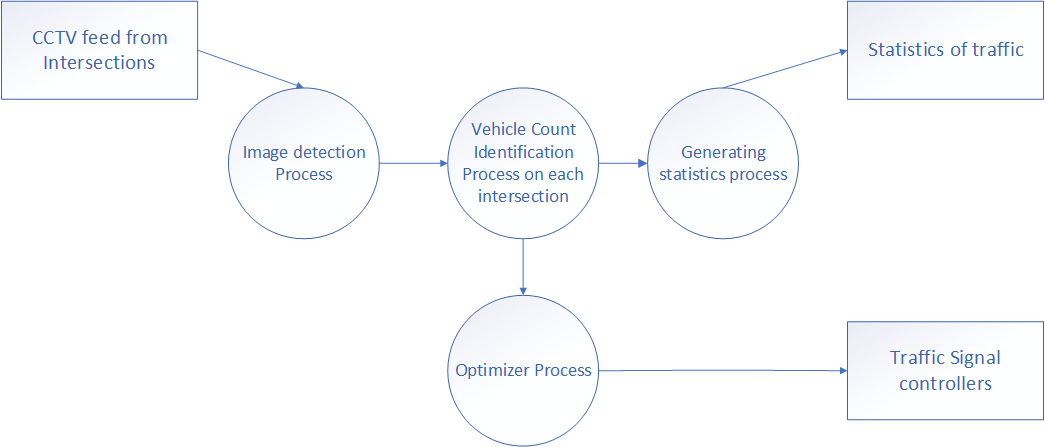
\includegraphics[width=6.8in,height=2.3in]{./Diagrams/PNG/dfd1}
		\caption{Level 1 Data Flow Diagram}
	\end{figure}
	
	
	\section{Summary}
	\hspace*{0.5in} This chapter discusses the system architecture, operating environment and the software attributes which describe the scope of the project.
	%*****************************Chapter 6******************
	
	\chapter{Modeling}
	
	\hspace*{0.5in} This chapter includes the various modeling techniques which describes the various users of the Artificially Intelligent Traffic Management System. It also describes the functionality of the different features of the Artificially Intelligent Traffic Management System.
	
	\section{Use Case Diagram}
	\hspace*{0.5in} A use case diagram is a type of behavioral diagram defined by the UML created from a use case analysis. Its purpose is to present a graphical overview of the functionality provided by a system in terms of actors, their goals represented as use case and any dependencies between those use cases.\\
	\hspace*{0.5in}Four modeling elements make up the use case diagram; these are:\\
	\begin{itemize}
		\item{\textbf{Actors:} Actors refer to a type of users, users are people who use the system. In this case traffic officers are the users of the framework and application}
		\item{\textbf{Use cases:} A use case defines behavioral features of a system. Each use case is named using a verb phrase that express a goal of the system. The name may appear inside or outside the ellipse.}
		\item{\textbf{Associations:} An association is a relationship between an actor and a use case. The relationship is represented by a line between an actor and a use case.}
		\item{\textbf{The include relationship:} It is analogous to a call between objects. One use case requires some type of behavior which is fully defined in  another use case.}
		\item{\textbf{The extend relationship:} It is intended for adding parts to existing use cases as well as for modeling optional system services}
	\end{itemize}
	The usecase diagram for proposed system is given in the figure 6.1.
	\begin{figure}[H]
		\centering
		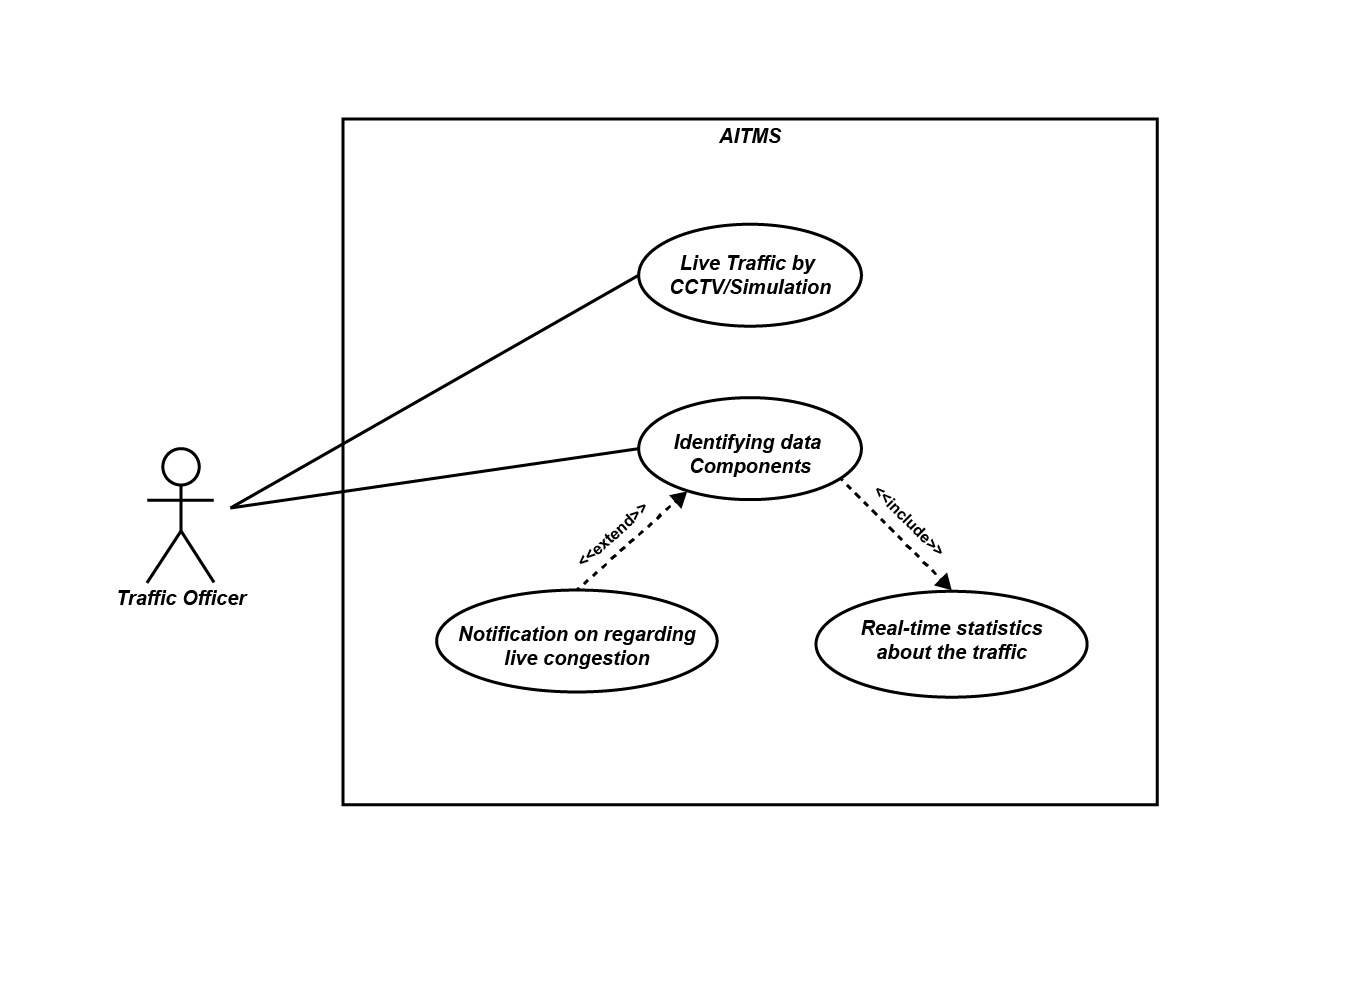
\includegraphics[width=5.5 in]{./Diagrams/PNG/uml}
		\caption{Use Case Diagram}
	\end{figure}
	
	\begin{comment}
		\newpage
		\section{Class Diagram}
		\hspace*{0.5in}The class diagram shows the building blocks of any object oriented system. Class diagram depicts a static view of the model or part of the model, describing what attributes and behavior it has rather that the detailing the methods of achieving operations. Class diagrams are most useful in illustrating relationships between classes and interfaces. Generalizations, aggregations, and associations are all valuable in reflecting interface, composition or usage and connections receptively.\\
		\hspace*{0.5in}The Figure 6.2 illustrates aggregation relationships between classes. The lighter aggregation indicates that the class ObjectExplorer used ThumbNail, but does not necessarily contain an instance of it.The strong, composite aggregations by the other connectors indicate ownership or containment of the source classes by the target. Class, for example VideoPlayer  values will be contained in TableOfContents.
	\end{comment}
	\newpage
	\section{Activity Diagram}
	\hspace*{0.5in}Use cases show what your system should do. Activity diagrams allow you to specify how your system will accomplish its goals. Activity diagrams show high-level actions chained together to represent a process occurring in your system. An activity diagram is essentially a flowchart, showing flow of control from activity to activity. Unlike a traditional flowchart, an activity diagram shows concurrency as well as branches of control. Activity diagrams focus on the dynamic flow of a system.\\
	\begin{comment}\hspace*{0.5in}An activity is the process being modeled, such as using the M-Learning application. An action is a step in the overall activity, such as select subject, select topic. The flow of the activity is shown using arrowed lines called edges or paths. The arrowhead on an activity edge shows the direction of flow from one action to the next. A line going into a node is called as an incoming edge, and a line exiting a node is called an outgoing edge. Fork Node is used to show the parallel or concurrent actions. Fork has single incoming flows and multiple outgoing flows. The join means that all incoming actions must finish before the flow can proceed past the join. Join has multiple incoming flows and single outgoing flow.
	\end{comment}
	The activity diagram for proposed system is given in the figure 6.2.
	\begin{figure}[H]
		\centering
		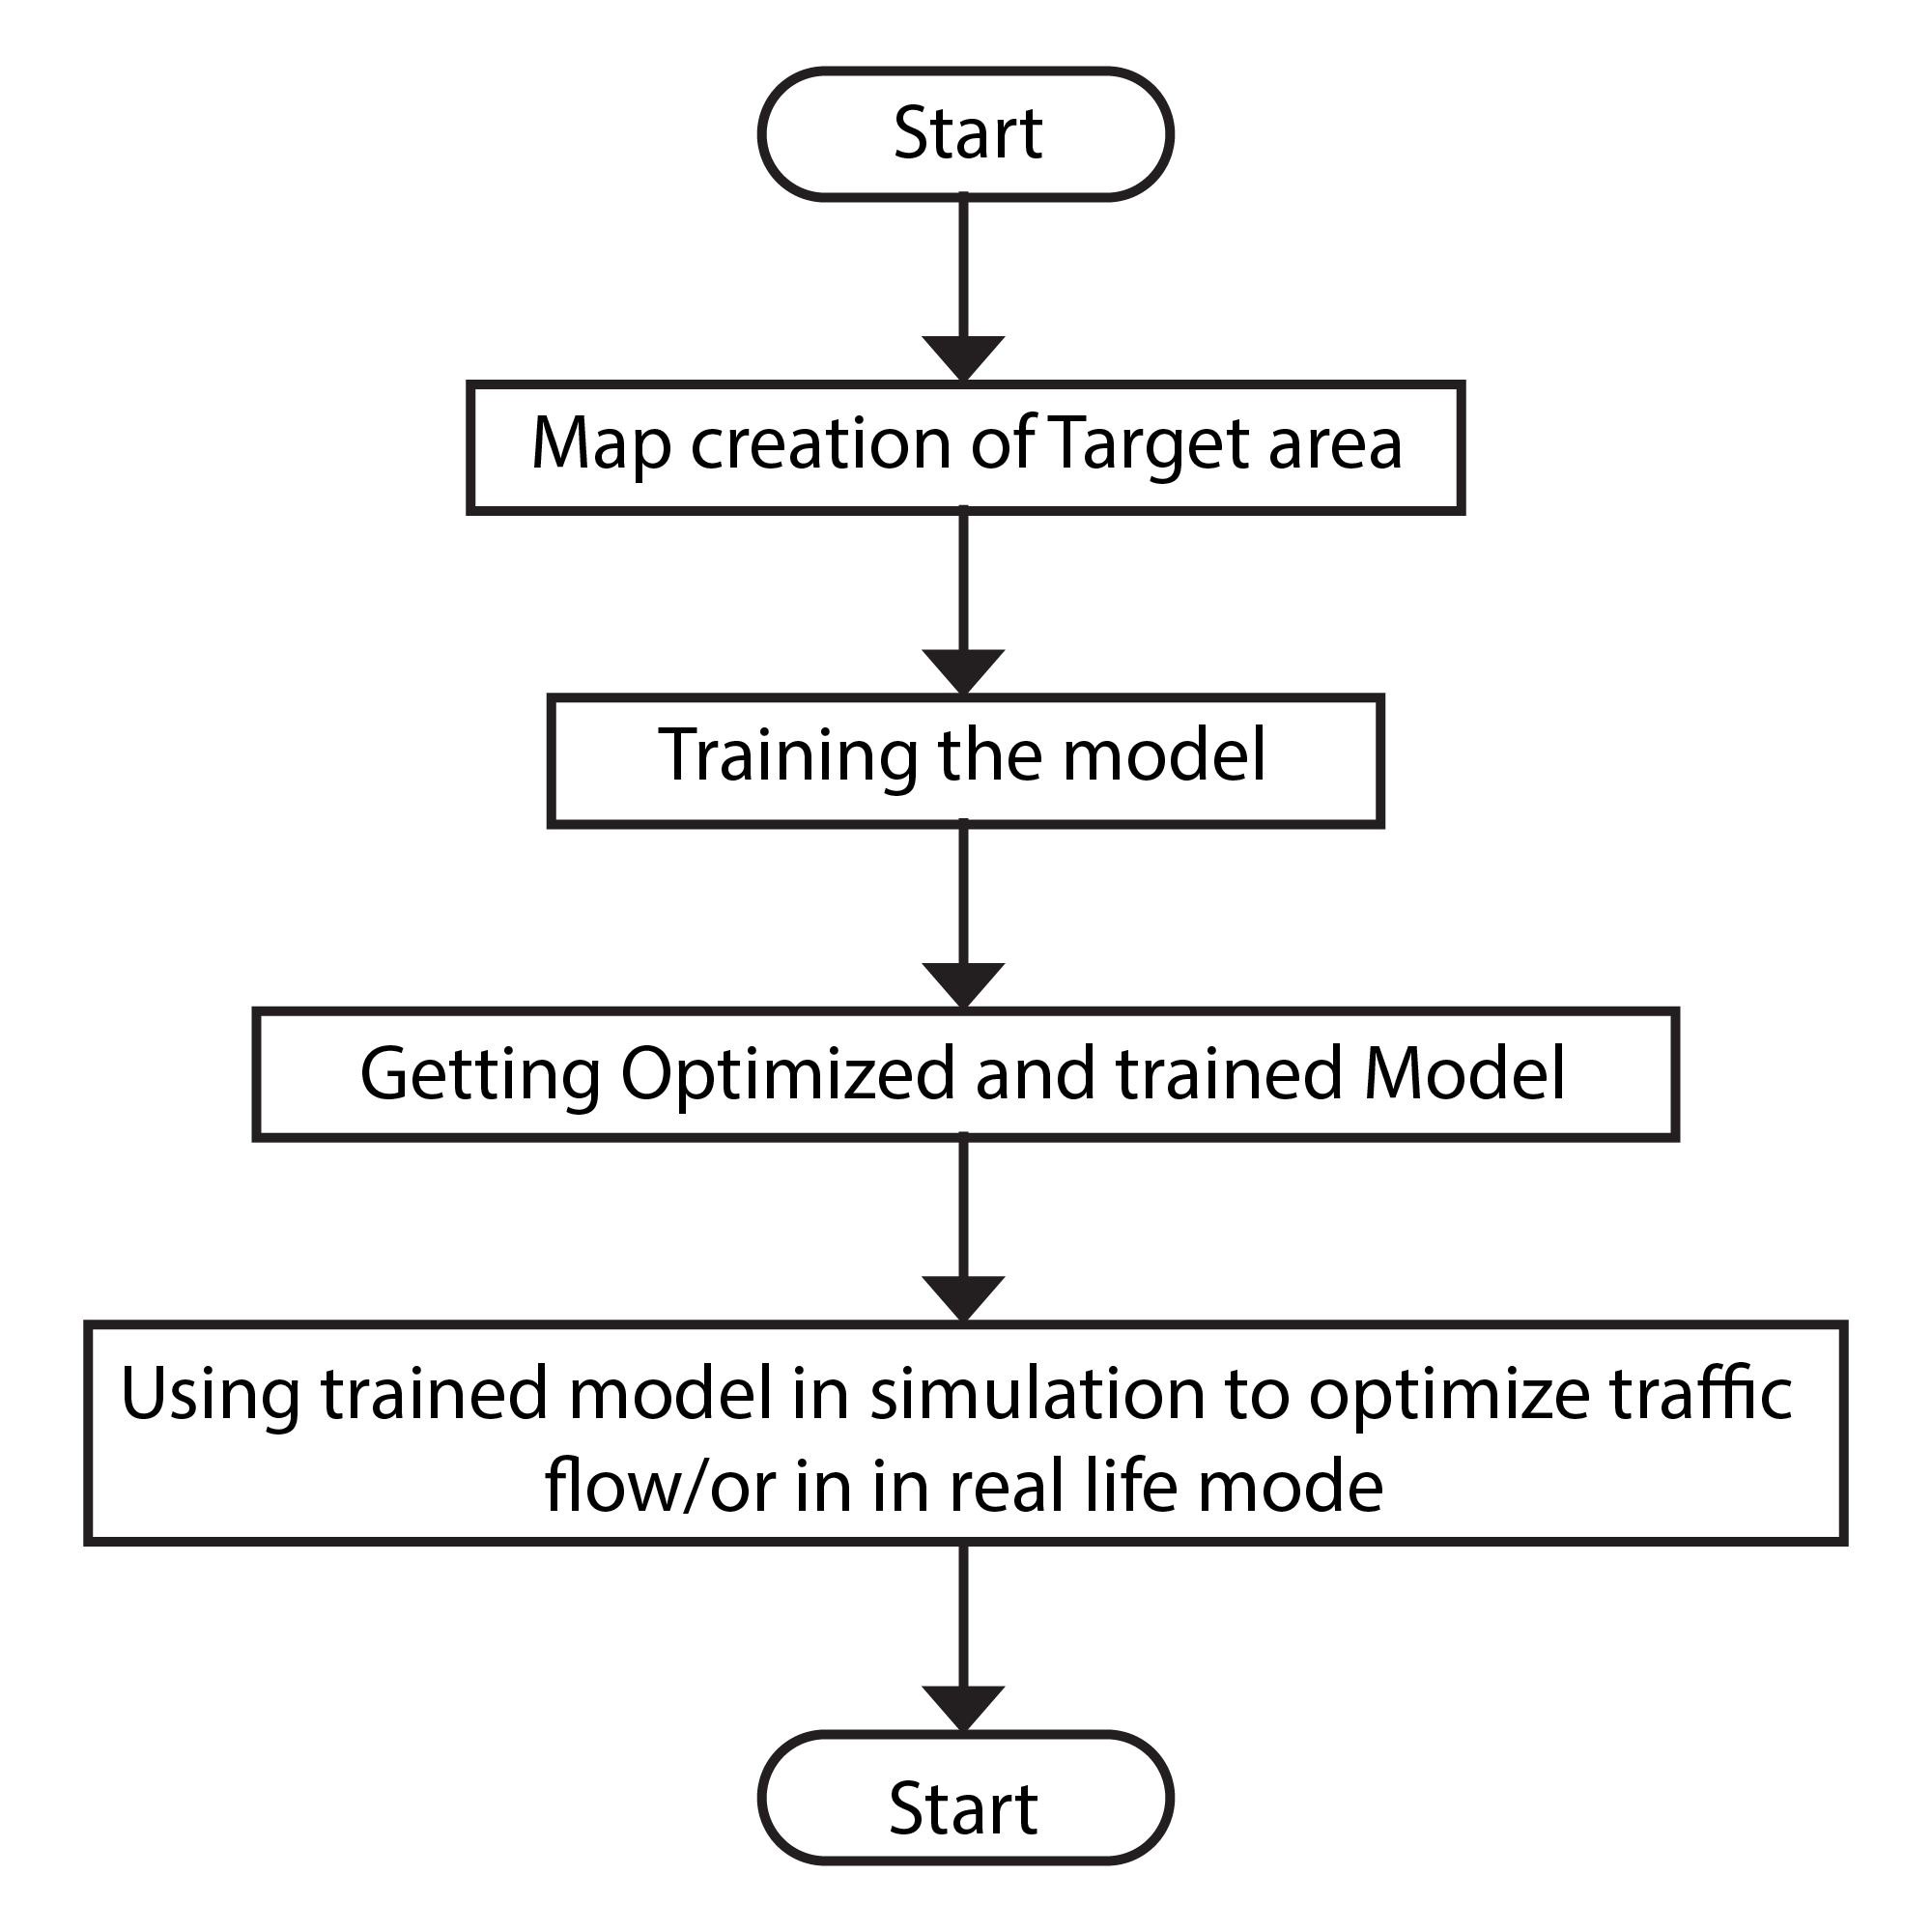
\includegraphics[height=5in]{./Diagrams/PNG/flow}
		\caption{Activity Diagram}
	\end{figure}
	\newpage
	
	\begin{comment}	
		\section{Sequence Diagram}
		\hspace*{0.5in}The sequence diagram is used primarily to show the interactions between objects in the sequential order that those interactions occur. Developers typically think sequence diagrams were meant exclusively for them. However, an organization's business staff can find sequence diagrams useful to communicate how the business currently works by showing how various business objects interact.Sequence diagrams illustrate how objects interact with each other. They focus on message sequences, that is, how messages are sent and received between a number of objects. The main purpose of sequence diagram is to show the order of events between the parts of system that are involved in particular interaction.\\
		\hspace*{0.5in}The basic element of sequence diagram is collection of participants, that is, the parts of the system that interact with each other during the sequence. The participants are arranged horizontally with no two participants overlapping each other. in Figure 6.4 developer, framework, applications are some examples of participants. A message is communication between objects that conveys information with the expectation that action will be taken. An event is any point in an interaction where something occurs. Message can flow in whatever direction makes sense for the required interaction from left to right, right to left, or even back to the Message Caller itself.
		
		
		\newpage
		\section{Package Diagram}
		\hspace*{0.5in} Package diagrams are used to reflect the organizations of packages and their elements, and provide a visualization of their corresponding name space. Following are the elemts of package diagram:
		\begin{itemize}
			\item{\textbf{Package:} A package is a namespace as well as an element that can be contained in other package's namespace. A package can own or merge with other package, and its elements can be imported into a package's namespace.}
			\item{\textbf{Class:} A class is a representation of objects, that reflects their structure and behavior within the system. It is a template from which actual running instances are created. A class may have attributes and methods.}
			\item{\textbf{Interface:} An interface is a specification of behavior that implements agree to meet, it is a contract. By implementing an interface, classes are guaranteed to support a required behavior.}
			\item{\textbf{Object:} An object is an instance of a class at runtime. Objects are often used in analysis to represent the numerous artifacts and items that exist in any business.}
			\item{\textbf{Table:} A table is a stereotyped class. It is drawn with a small table icon in the upper right corner. A table element has special properties dialog with settings for database type and ability to set column information and data related operations such as triggers and indices.}
		\end{itemize}
		
		
		\newpage
		\section{State Machine Diagram}
		\hspace*{0.5in}A state machine diagram models the behavior of a single object, specifying the sequence of events that an object goes through during its lifetime in response to events. In figure 6.6, the state machine diagram shows the states the that a video or an audio file goes through during its lifetime. The file can be in one of the four states Play, Pause, Seek or Stop. It can respond to the events Play, Pause, Seek and Stop. Notice that not all events are valid in all states. For example; if a video is stopped, you cannot pause it until you play it. Also notice that a state transition can have a guard condition attached. If the file is stopped it can only respond to the play event.
		
		\newpage
		\section{Object Diagram}
		\hspace*{0.5in}In UML, an object diagram is a diagram that shows complete or partial view of the structure of a modeled system at a specific time. This snapshot focuses on some particular set of object instances and attributes and link between instances. Object diagrams are useful in understanding class diagrams. They don't show anything architecturally different to class diagram, but reflects multiplicity and roles. Basically an object diagram shows a set of objects and their relationships at a specific point in time.\\
		\hspace*{0.5in}To draw an object diagram, the first thing is to add the actual objects themselves. Object notation is actually very simple if one is familiar with class notations; an object is shown with a rectangle just like a class, but to show that this is an instance of a class rather than the class itself, the title is underlined. An object is representation of an entity. Each object in  a system has three characteristics: state, behavior and identity. The state of an object is one of the possible conditions in which it may exist, the state of an object typically changes over time.
		\newpage
		
		\end{comment}
		
		\newpage
		\section{Component Diagram}
		\hspace*{0.5in}Component diagram are one of the two kinds of diagrams found in modeling the physical aspects of object oriented systems. A component diagram shows organization and dependencies among set of components. Component diagram can be seen to model the static implementation view of a system. This involves modeling the physical things that resides on a node, such as executables, libraries, tables, files and documents.\\
		\hspace*{0.5in}Component diagram shows a set of components and their relationships. Graphically a component diagram is a collection of vertices and arcs. Component diagrams commonly contain,
		%\begin{itemize}
		%	\item{\textbf{Components}}
		%	\item{\textbf{Interfaces}}
		%	\item{\textbf{Dependency, generalization, association and realization relationships.}}
		%\end{itemize}
		\begin{figure}[H]
			\centering
			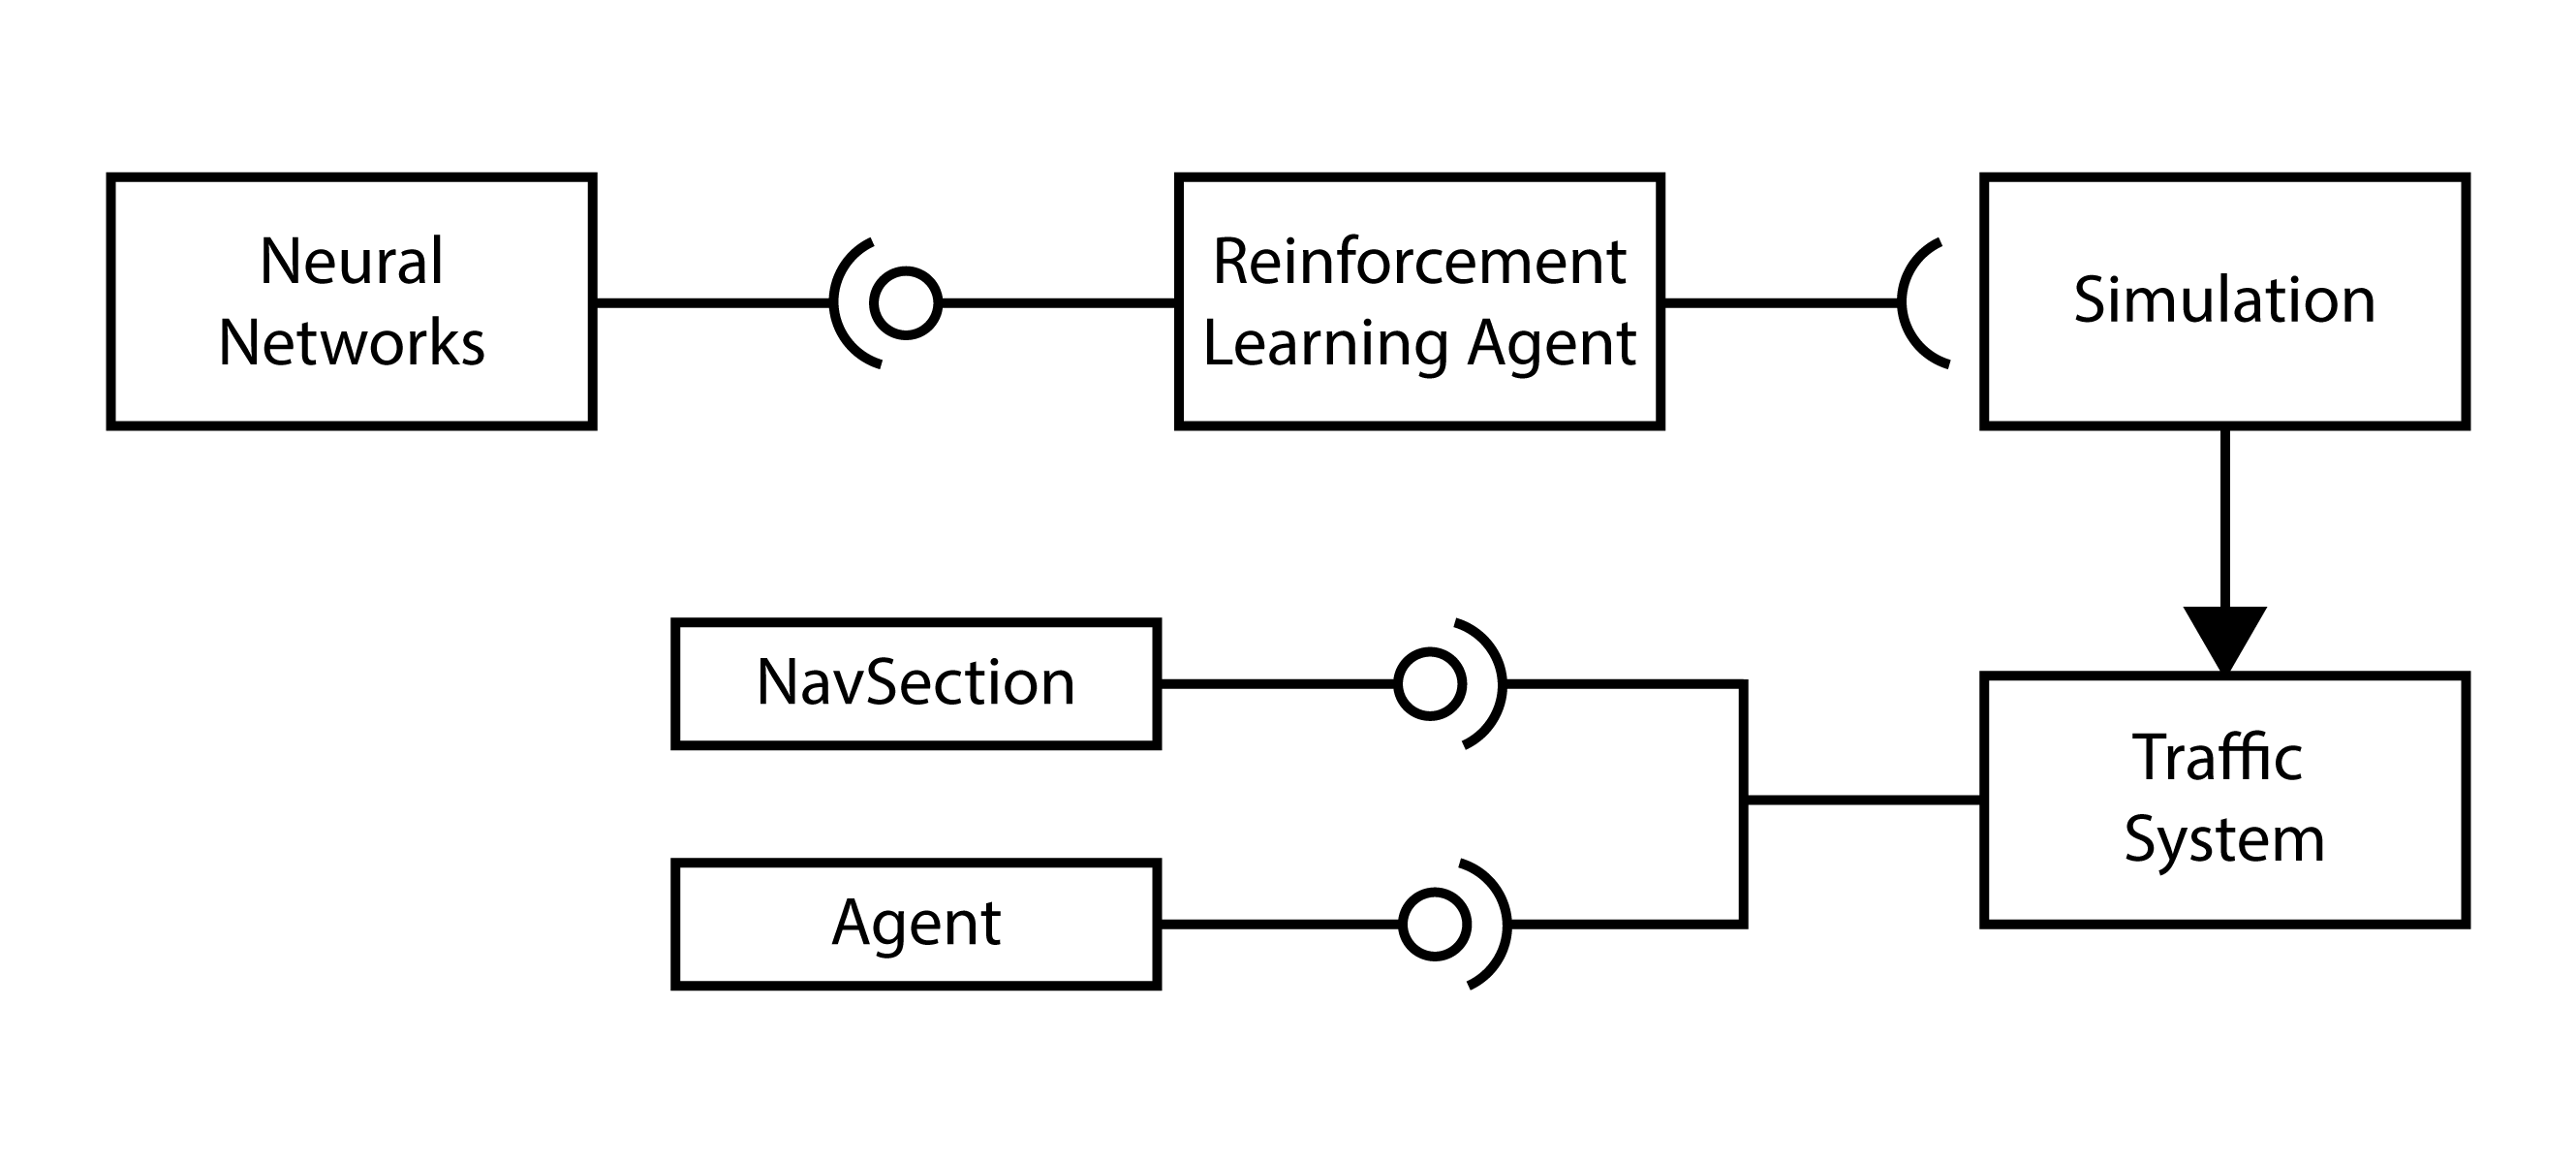
\includegraphics[width=5.6in]{./Diagrams/PNG/cc}
			\caption{Component Diagram}
		\end{figure}
		\newpage
		\begin{comment}
		\newpage
		\section{Deployment Diagram}
		\hspace*{0.5in}he deployment diagram depicts the runtime architecture of devices, execution environments and artifacts that reside in this architecture. It is the ultimate physical description of the system topology, describing the structure of the hardware units and the software taht executes on each unit. The deployment diagram shows how a system will be physically deployed in the hardware environment. Its purpose is to show where the different components of the system will physically run and how they will communicate with each other.
	\end{comment}
	
	\section{Summary}
	\hspace*{0.5in}Thus the various modeling techniques used for the design of Artificially Intelligent Traffic Management System were seen in this chapter.
	
	
	
		
		%*****************************Chapter 7******************
		\chapter{Implementation and Results}
		\hspace*{0.5in}This chapter consists of the various implementation details and snapshots of the Artificially Intelligent Traffic Management System.
		
		\section{Implementation Details}
		
		\begin{itemize}
			
			\item{\textbf{Simulation} The Simulation is one of the most important features provided by AITMS. Simulation provides creation of maps of traffic system, it also helps in simulating real-time traffic and visualizing traffic densities. It is implemented in Unity3D. Simulation is further divide into many smaller modules below. \begin{itemize}
			\item{\textbf{NavMesh Module:} The NavMesh represents the area where the center of the agent can move. 
			\begin{figure}[H]
				\centering
				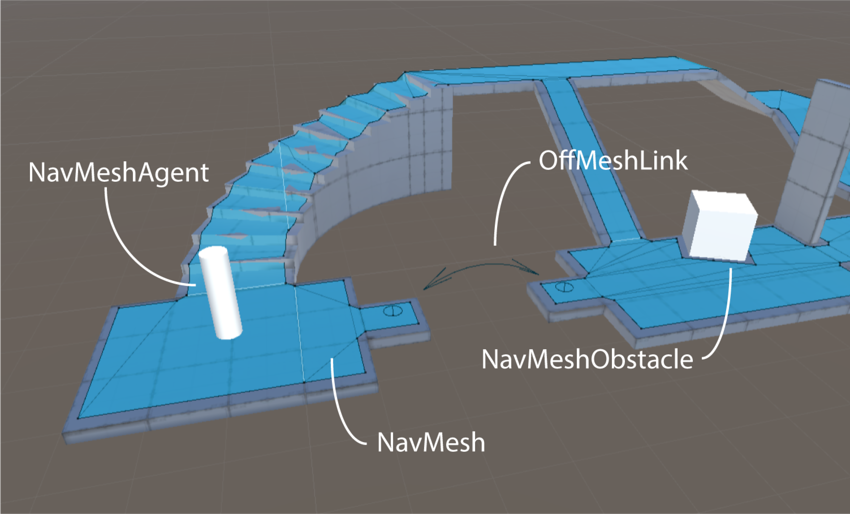
\includegraphics[width=3 in]{./Diagrams/PNG/NavMeshModule}
				\caption{NavMesh Components}
			\end{figure}
			Conceptually, it doesn’t matter whether you regard the agent as a point on a shrunken NavMesh or a circle on a full-size NavMesh since the two are equivalent.NavMesh module help in baking the path for agents to run on the guided path which makes it easier to simulate real-time traffic.}
			
			\item{\textbf{Agent Module:} In this module, Agents(Different vehicles such as cars, buses, trucks etc) prefabs are available. These agents prefabs are used to simulate vehicles in the real-time traffic system.}
			\item{\textbf{NavSection Module:} In this module, NavSection prefabs are available which helps in designing realistic maps. It includes many predefined NavSection prefabs for single lane, double lane, bridges, highway roads etc. }
			\item{\textbf{Junction Observables Module:} This module observes the current state and environment of the juntions and passes it to RL Agent. This module is used only when the model is training. It outputs current phase, phase count, phase timing  to RL Agent.}
			\end{itemize}			 
			}
			
			
			
			\item{\textbf{Reinforcement Learning}}\\
			\hspace*{0.5in}It is an area of machine learning concerned with how intelligent agents ought to take actions in an environment in order to maximize the notion of cumulative reward.\\
			\hspace*{0.5in}The model is trained using MLAgents toolkit in Unity. Training is set up by adding the JunctionRLAgent script to the Junction object which is to be trained. JunctionRLAgent consists of the reward mechanism which penalizes (i.e. negative reward) the model based on halt duration of vehicles that pass through the junction and the number of vehicles remaining in a lane after its phase. \\
			\hspace*{0.5in}The aim of training would be to minimize these parameters, hence model must be able to reduce the overall waiting time of vehicles and at the same time provide optimal green time for all waiting vehicles of the current phase to pass through. The input of the model is obtained from the Junction Observables Module explained above.
			
		\end{itemize}
	
		\newpage
		\section{Steps for Training a Smart Traffic Signal}
		\hspace*{0.5 in}Following steps are to be followed to train a smart signal from scratch using AITMS.

		\begin{minipage}[t]{0.05\textwidth} 

		\end{minipage}
		\hfill
		\begin{minipage}[t]{0.95\textwidth} 
		
		\newcounter{number}
			\addtocounter{number}{1}
			\thenumber . Create a new scene in Unity3D; Create a road map consisting junctions by simply dragging and dropping NavSection prefabs. Finally click bake to complete map creation.\\
			\addtocounter{number}{1}
			\thenumber . Tune generalized parameters (speed limits, connections, etc.) of placed NavSection components and vehicle prefabs as desired.\\
			\addtocounter{number}{1}
			\thenumber . Add JunctionRLAgent script to junctions which are to be trained. Optionally, pass GlobalObservables if inference from other junctions is required. If a custom reward mechanism is desired, it can be implemented in the Junction script.\\
			\addtocounter{number}{1}
			\thenumber . Edit training configuration file as desired.\\
			\addtocounter{number}{1}
			\thenumber . Start an instance of MLAgents using the configuration file and hit play in Unity.\\
			\addtocounter{number}{1}
			\thenumber . Let model train for atleast a couple thousand steps, this step takes the longest time depending on size of map, complexity of reward mechanism and training configuration. Training can be visualized as it happens using tensorboard.\\
			\addtocounter{number}{1}
			\thenumber . Attach trained model (".onnx" file) to Junction in scene and evaluate by enabling log option in AITMS object.\\
			\end{minipage}
		\section{Training Configuration}
		\hspace*{0.5 in}MLAgents models are trained based on a configuration file having a ".yaml" extension. Properties for each model such as trainer type, number of layers, etc. are defined in this file. 
		It allows tuning hyperparameters and environment settings. For more details check out the MLAgents documentation page.
		
		\newpage
		\section{Reward Mechanism}
		\hspace*{0.5 in}Reward mechanism plays a key role in training reinforcement learning models. The aim of reinforcement learning is to maximize rewards obtained through each decision made. The default reward function of AITMS is given as follows\\ 
		\hspace*{1 in}$\mathbf{Reward = - (\ AvgHaltTime \times LaneCount )\ }$\\
		where, AvgHaltTime is the average of waiting time of all the vehicles that have passed through the junction in current phase and LaneCount is the amount of vehicles (value is scaled using maxmin scaling) remaining after end of current phase. Reward is calculated at the end of each phase.\\
		\hspace*{0.5 in} Since reward is negative, the model tries to minimize the magnitude during training. Hence, through training, the model should be able to reduce average waiting time of the vehicle as well as set optimal phase time such that maximum waiting vehicles pass through during every phase.\\
		\section{Model Architectures}
		\hspace*{0.5 in} AITMS models can be trained in the following possible structures.
		\begin{itemize}
			\item{The same model is attached to multiple junctions. Hence junctions share a generalized model.}
			\item{Different model is attached to each junction. Hence each model is specialized to optimize its own junction.}
			\item{Hybrid, i.e. a combination of the above two structures.}
		\end{itemize}
		\newpage
		\section{Results}
		\hspace*{0.5in}The snapshots below are taken on the desktop device itself having Windows 11 or Linux based operating system, screen of 17 inches with a resolution of 1900 x 1080.\\
		
		
		
		\hspace*{0.5in}Following are the snapshots of AITMS:
		
		\begin{figure}[H]
			\centering
			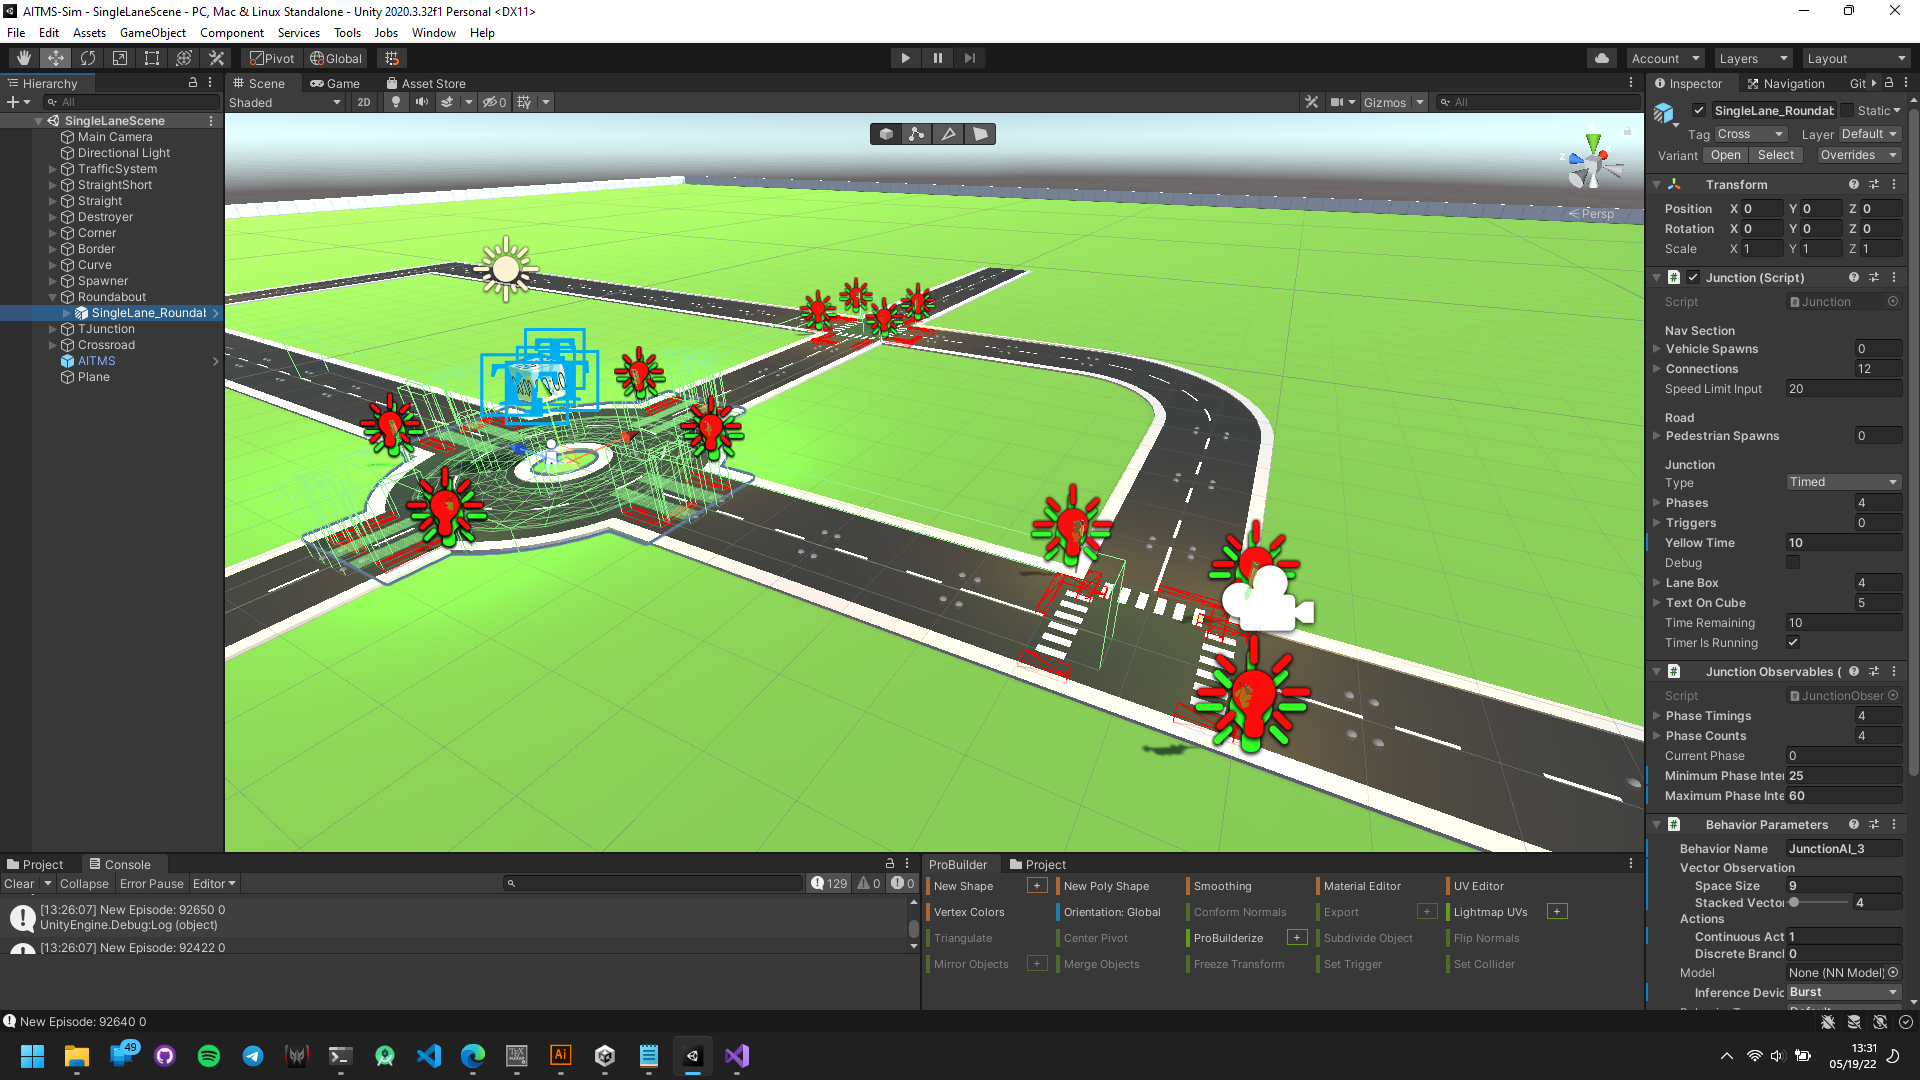
\includegraphics[width=6in]{./Diagrams/PNG/scene}
			\caption{AITMS Scene Creation Screen}
		\end{figure}
		
		\begin{figure}[H]
			\centering
			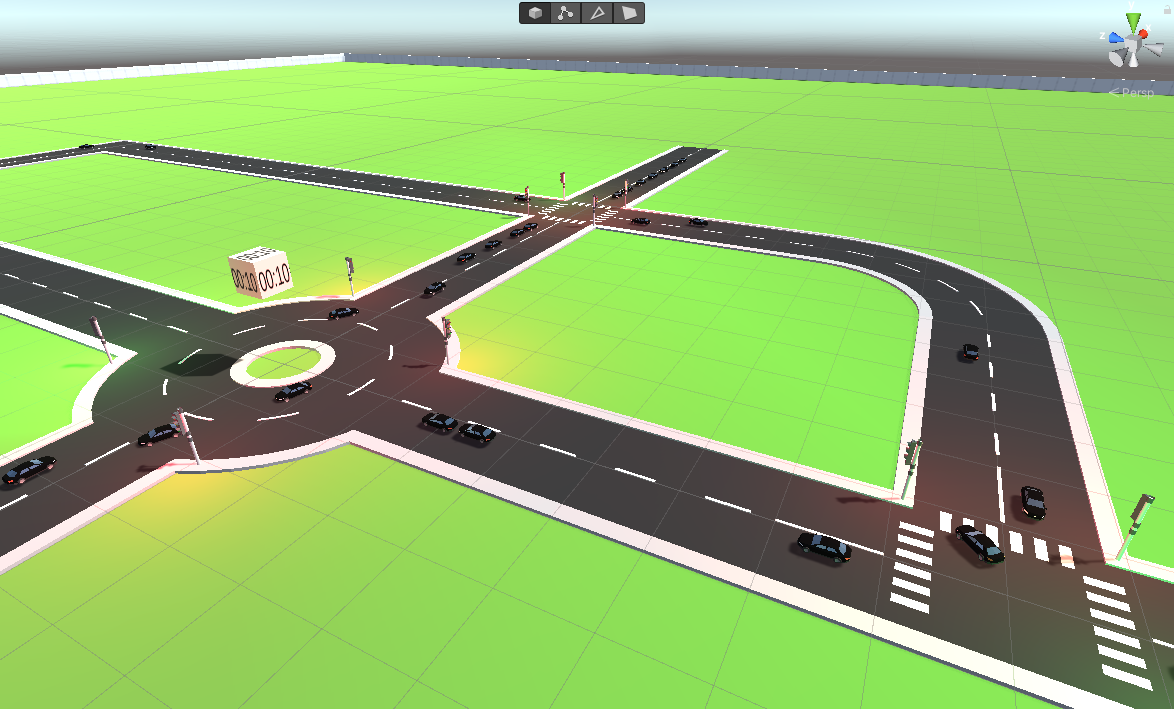
\includegraphics[width=6in]{./Diagrams/PNG/cross}
			\caption{AITMS Simulation Screen}
		\end{figure}
		
		\begin{figure}[H]
			\centering
			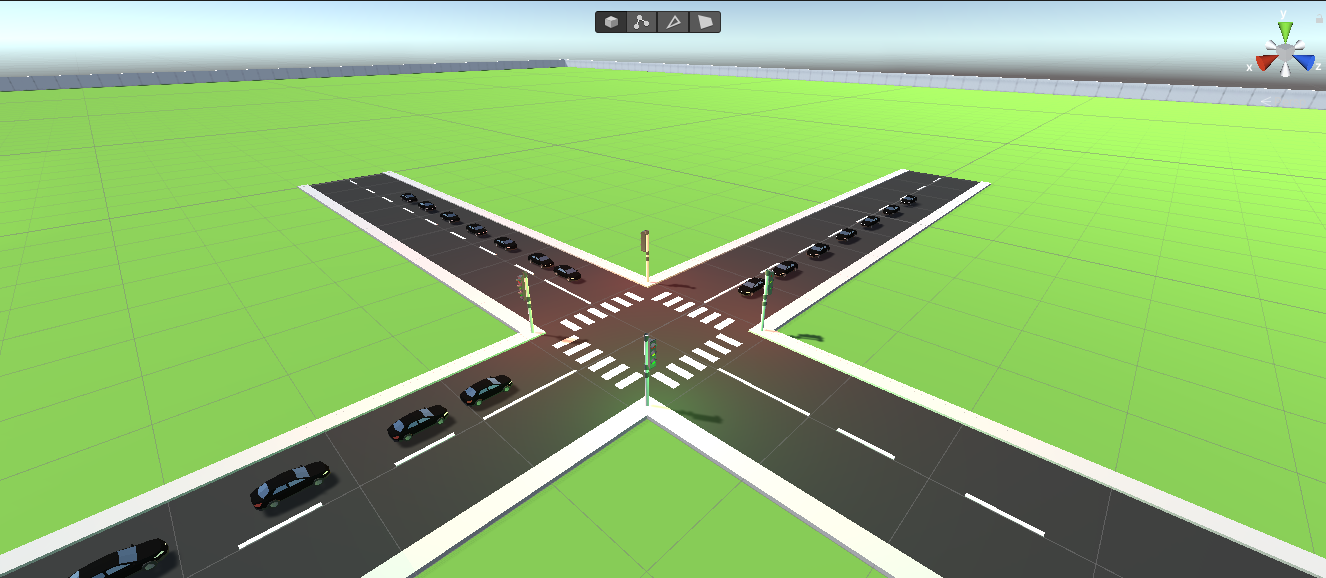
\includegraphics[width=6in]{./Diagrams/PNG/licescene2}
			\caption{AITMS Simulation Screen (Intersection)}
		\end{figure}
		
		\begin{figure}[H]
			\centering
			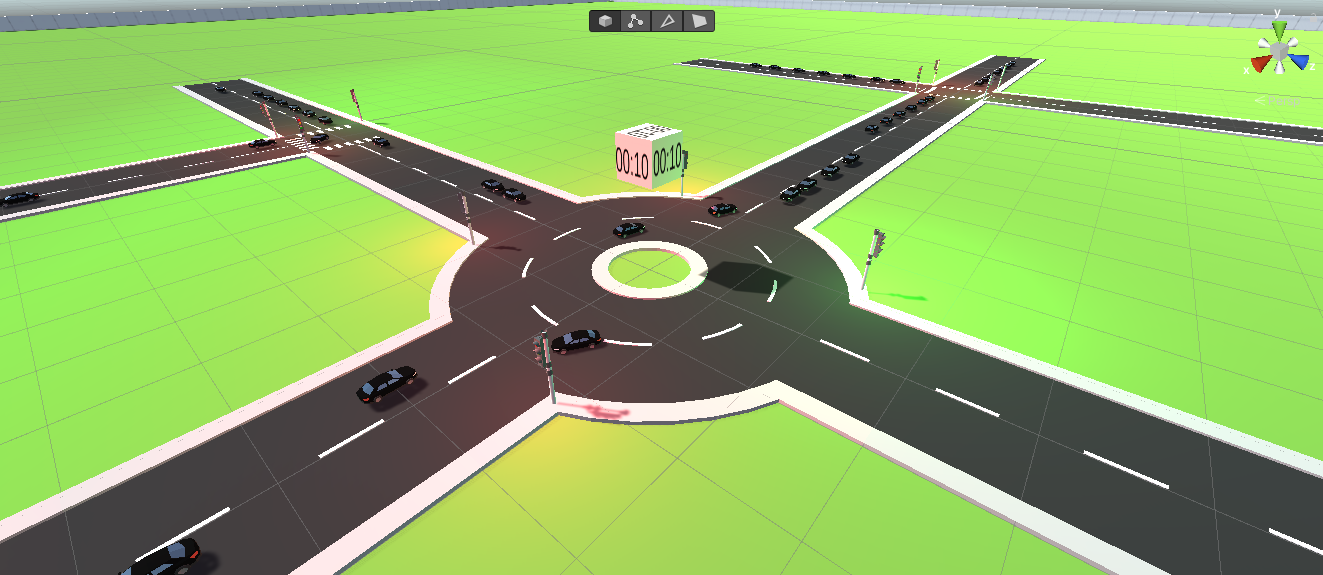
\includegraphics[width=6in]{./Diagrams/PNG/livescene}
			\caption{AITMS Simulation Screen (Roundabout)}
		\end{figure}
		
		\begin{figure}[H]
			\centering
			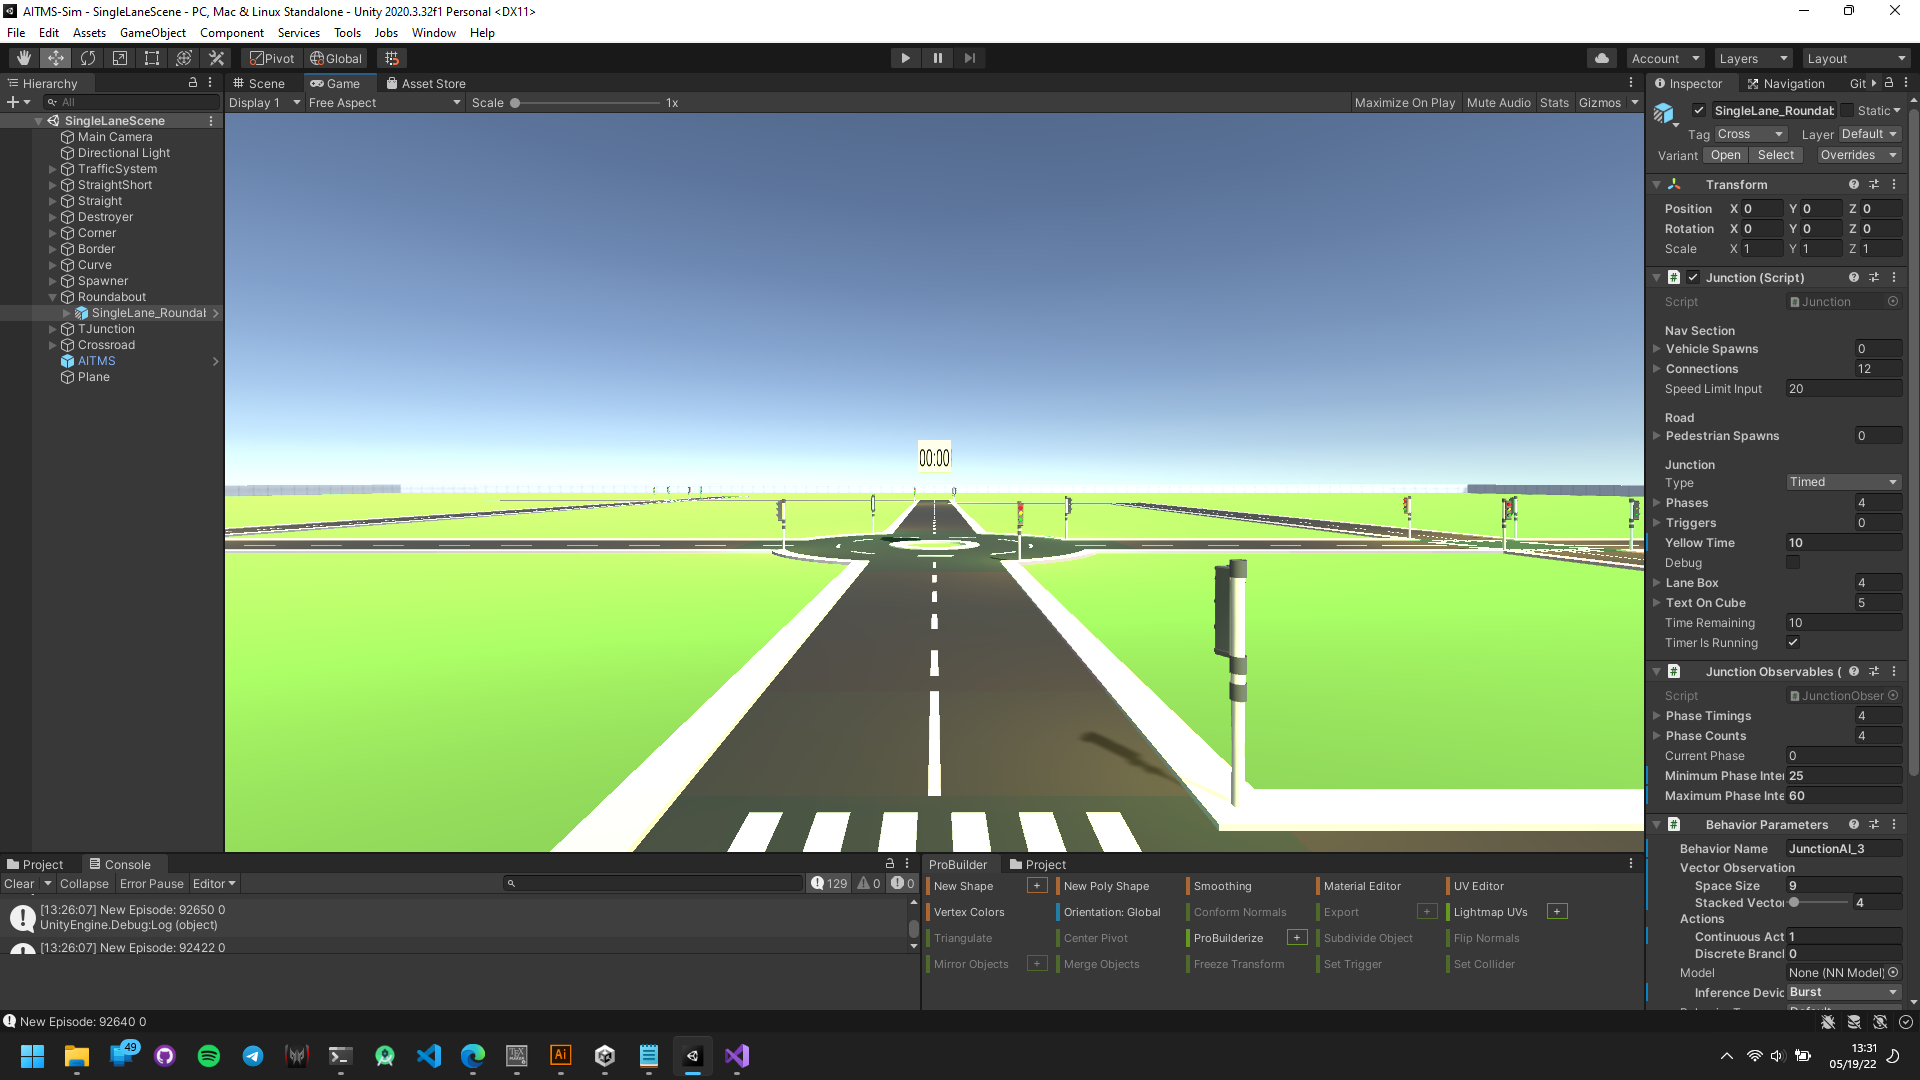
\includegraphics[width=6in]{./Diagrams/PNG/scene2}
			\caption{AITMS Game View Screen}
		\end{figure}
		
		\begin{figure}[H]
			\centering
			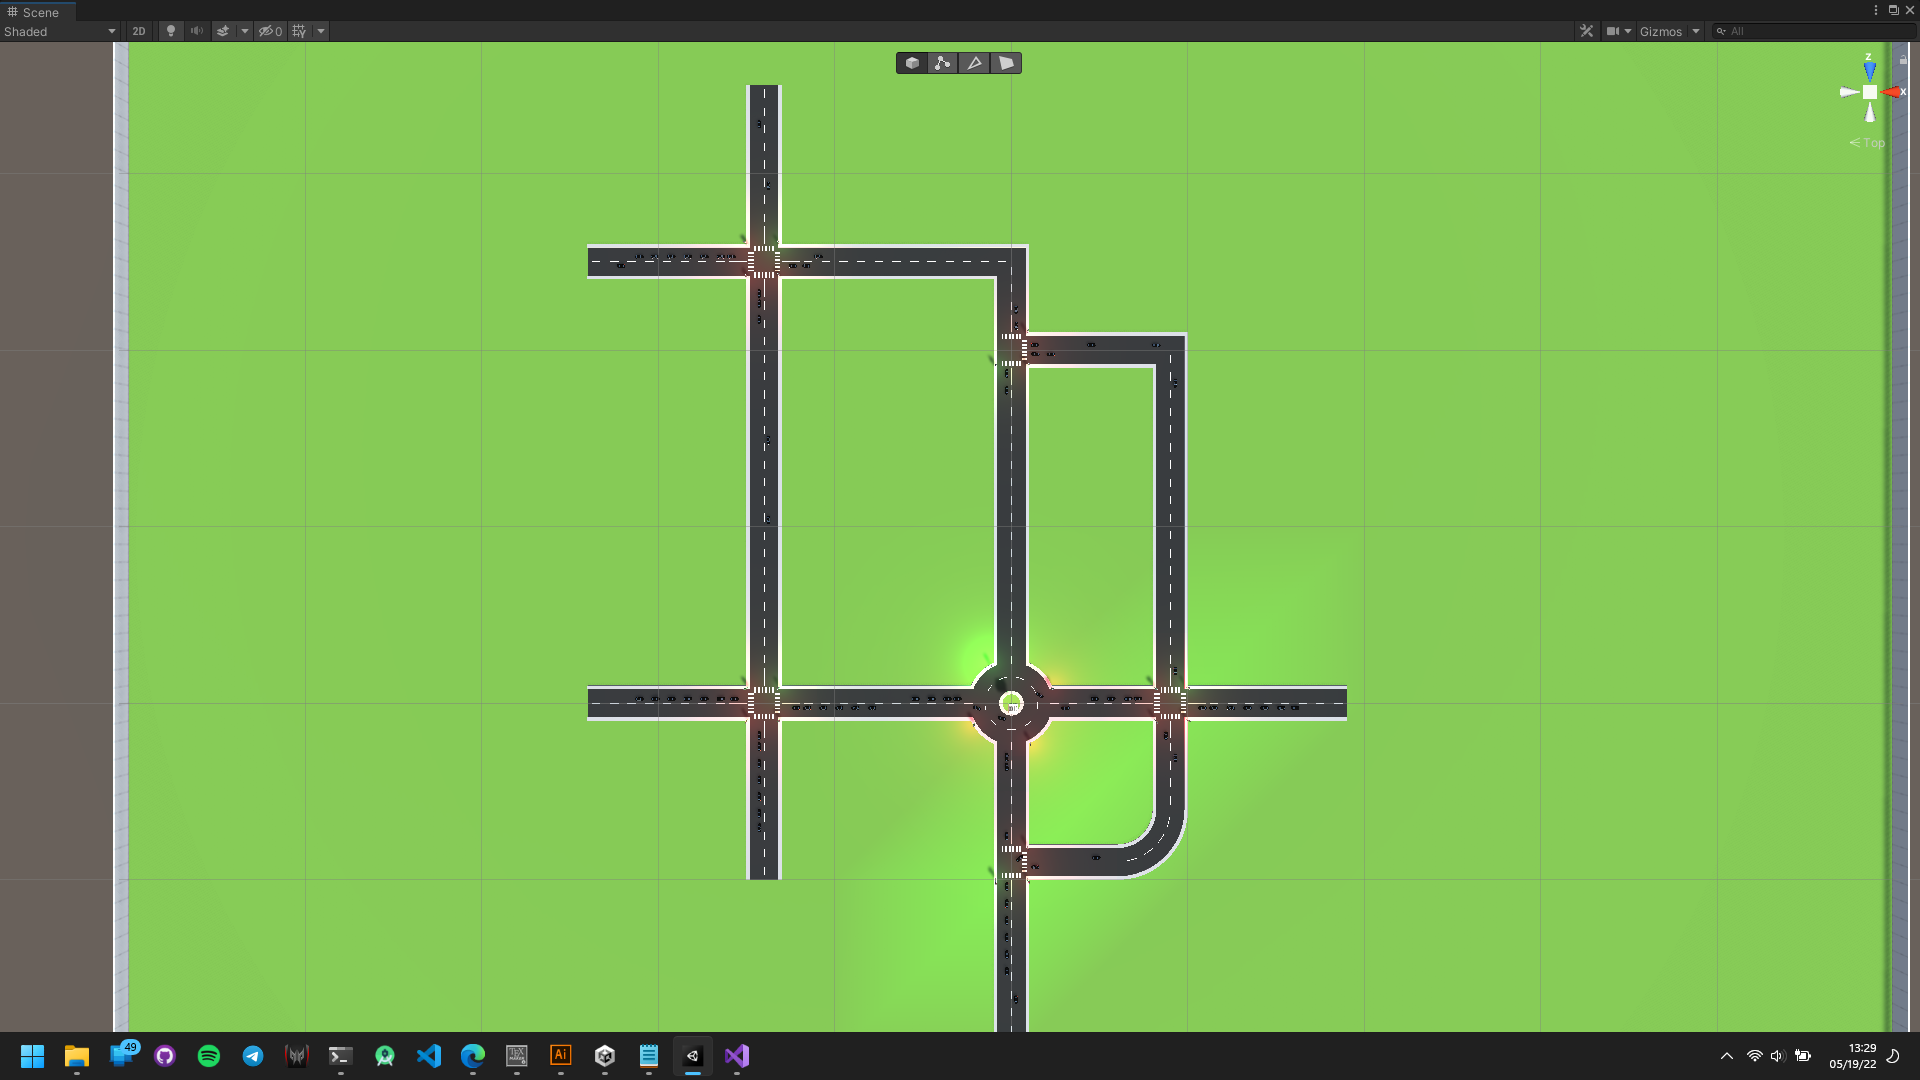
\includegraphics[width=6in]{./Diagrams/PNG/fulllive}
			\caption{AITMS Map Viewer}
		\end{figure}
		
		\begin{figure}[H]
			\centering
			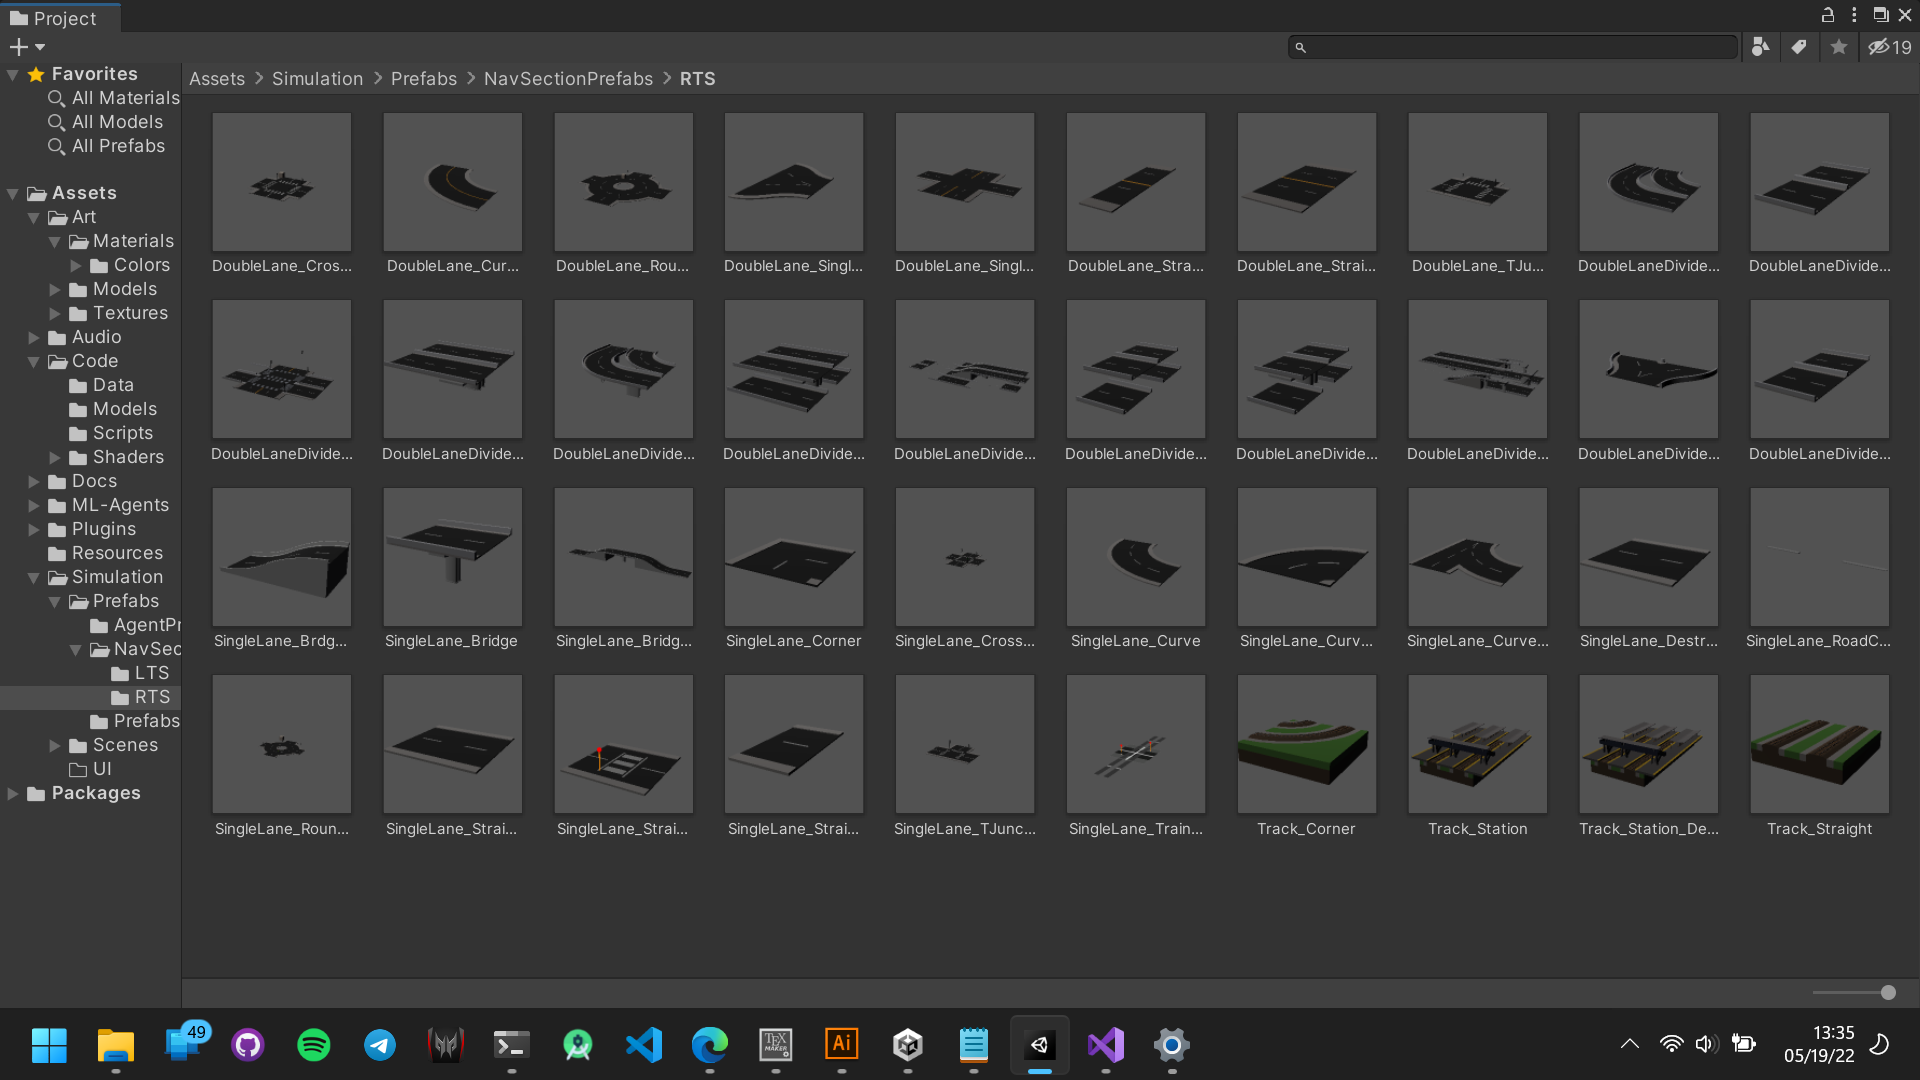
\includegraphics[width=6in]{./Diagrams/PNG/prefabs}
			\caption{AITMS NavSection Prefabs}
		\end{figure}
		
		\begin{figure}[H]
			\centering
			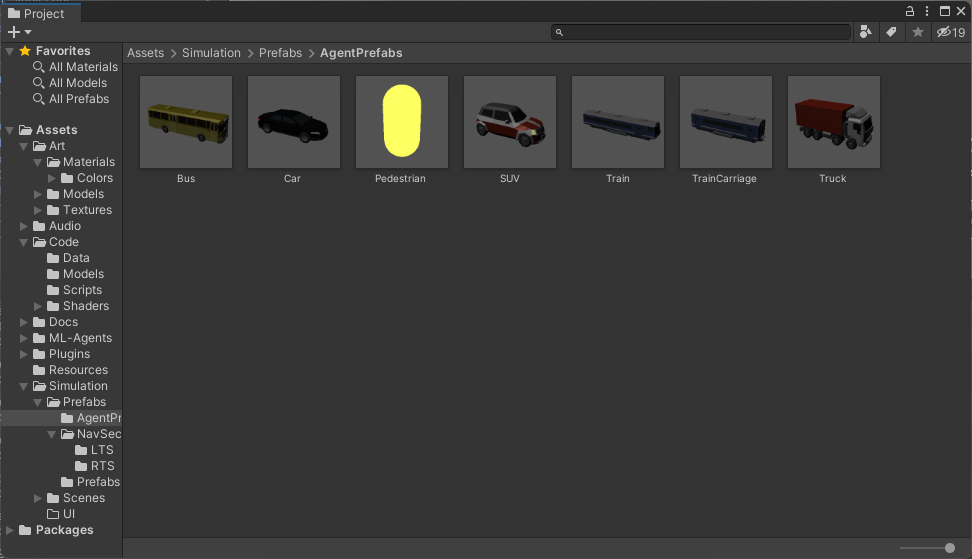
\includegraphics[width=6in]{./Diagrams/PNG/agent}
			\caption{AITMS Agent Prefabs}
		\end{figure}
		
		\begin{figure}[H]
			\centering
			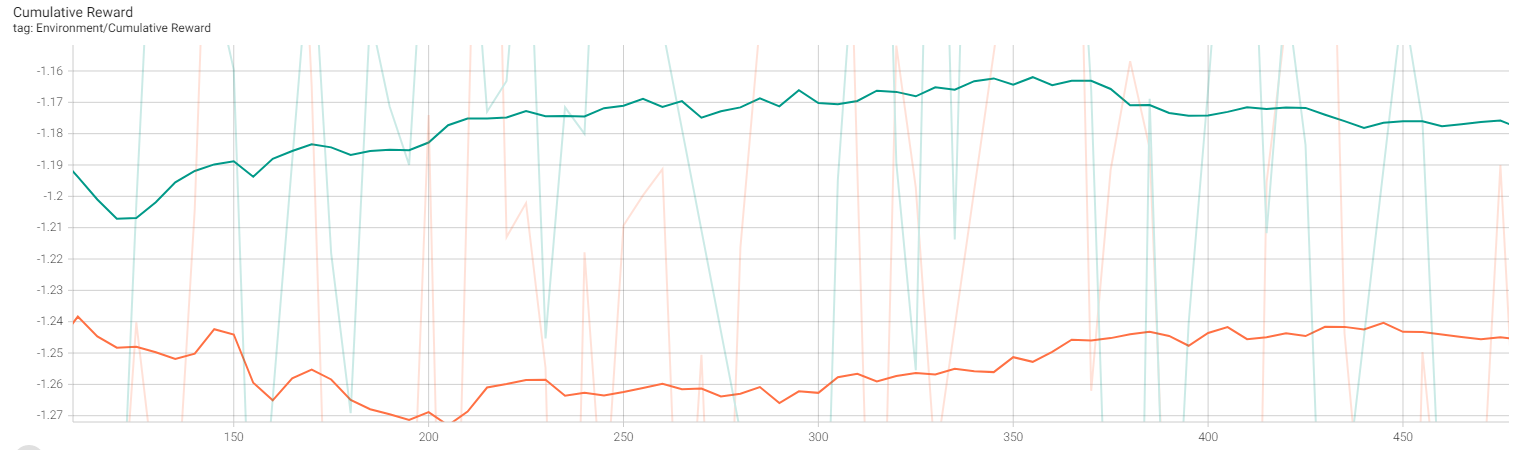
\includegraphics[width=6in]{./Diagrams/PNG/graph}
			\caption{AITMS Training Progress Graph (Rewards vs Steps)}
		\end{figure}		
		
		\begin{figure}[H]
			\centering
			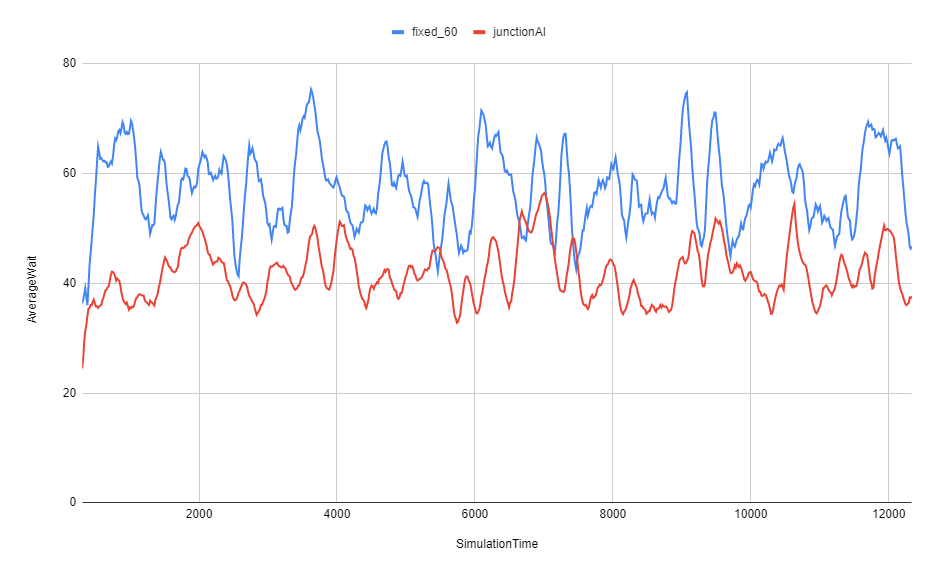
\includegraphics[width=6in]{./Diagrams/PNG/result}
			\caption{AITMS Training Result Graph (AvgWait vs SimulationTime) Showing Approximately 27 \% Improvement}
		\end{figure}	
		
		
		\section{Summary}
		\hspace*{0.5in}This chapter discusses the implementation details of the AITMS and also the implementation of various features included in the application. It also consists of the results in the form of snapshots of AITMS.
		
		%*****************************Chapter 8******************
		
		\chapter{Testing}
		\hspace*{0.5in}This chapter includes the details of Formal Technical Review meetings and describes the process carried during the review process. It also includes the Test Plan adopted for testing the Artificially Intelligent Traffic Management System and Application.
		\section{Formal Technical Review}
		\hspace*{0.5in}Formal Technical Reviews and Inspections of documents or software are performed to identify and remove defects. The Formal Technical Review of our project was carried at regular intervals in the form of stand-up meetings and brainstorming sessions conducted. The process included verification of the checklist which was developed for the review process ,the code review  checklist template is as follows:
		
		\begin{itemize}
			\item{\textbf{Does the code conform to Hungarian Notations?}}
			\item{\textbf{Is the code well-structured , consistent in style and consistently formatted?}}
			\item{\textbf{Are all variables properly defined with meaningful,consistent and clear names?}}
			\item{\textbf{Are there any redundant or unused variables?}}
			\item{\textbf{Does the code consist of comments ?}}
			\item{\textbf{Is the code error free?}}
			
		\end{itemize}
		
		\newcounter{num}
		
		\section{Test Plan}
		%\begin{longtable}{|p{3.5cm}|p{5cm}|p{3.5cm}|p{1.7cm}|} \hline
		\begin{longtable}{|p{0.6cm}|p{3.5cm}|p{5cm}|p{3.5cm}|p{1.7cm}|} \hline		
			\textbf{Sr.\newline no.} &\textbf{Module being Tested}	&\textbf{Expected Result}	&\textbf{Actual Result}	&\textbf{Verdict} \\\hline\hline

			\addtocounter{num}{1}
			\thenum&	
			Road assets designing&
			3D assets of road in Digital Asset Exchange(.dae) file format&
			3D assets were created using blender in .dae file format&
			PASS\\\hline
			
			\addtocounter{num}{1}
			\thenum&
			Core Traffic System&
			3D assets of road in Digital Asset Exchange(.dae) file format&
			3D assets were created using blender in .dae file format&
			PASS\\\hline
			
			\addtocounter{num}{1}
			\thenum&
			NavMesh Environtment Setup and Testing&
			Test if NavMesh package is working properly&
			NavMesh package working properly&
			PASS\\\hline			
			
			\addtocounter{num}{1}
			\thenum&
			NavConnection implementation to guide vehicle on road&
			If NavConnection module used to guide vehicle along road and intersections is working as per expectations&
			NavConnection module working properly and tested&
			PASS\\\hline
			
			\addtocounter{num}{1}
			\thenum&
			NavSection prefabs&
			NavSection prefabs which can be used to create maps in sumulation is working properly and aligning to the grid perfectly&
			NavSections preafabs for common road and intersections working as per expectations&
			PASS\\\hline
			
			\addtocounter{num}{1}
			\thenum&
			Vehicle(NavAgent) prefabs&
			NavAgents/Vehicles have realistic physics&
			NavAgents/Vehicles have physics as per expectations&
			PASS\\\hline
			
			\addtocounter{num}{1}
			\thenum&
			Road and Juntion Scripts&
			road and juntion scripts are followed by NavAgent&
			NavAgents following road and junction scripts as per expectations&
			PASS\\\hline
			
			\addtocounter{num}{1}
			\thenum&
			Simple Timed Traffic System&
			Implement a simple timed traffic system core model to navigate traffic, also to bake the NavMesh on runtime/pre-runtime and to manage vehicle pool&
			Implemented a simple traffic system using scripting and attached it to the relevant object in scene&
			PASS\\\hline
			
			\addtocounter{num}{1}
			\thenum&
			Map for simulation&
			If map can be created as per the need of traffic system&
			Map can be created using NavSection prefabs and is following traffic rules defined in traffic system&
			PASS\\\hline
			
			\addtocounter{num}{1}
			\thenum&
			Camera Module&
			Camera Module is working properly&
			Camera Module is working as per expectations&
			PASS\\\hline
			
			\addtocounter{num}{1}
			\thenum&
			Junction Observable Module&
			Junction Observable Module observing junctions properly and collecting data to forward to RL Agents&
			Junction Observable Module observing junction properly and environment as per expectations and ready to forward data to RL Agents&
			PASS\\\hline
			
			\addtocounter{num}{1}
			\thenum&
			RL Agents&
			Test if RL Agents interface is connected with Junction Observable module&
			RL Agents interface is linked properly with Junction Observable module and is ready to train RL models&
			PASS\\\hline
			
			\addtocounter{num}{1}
			\thenum&
			Verification of Reward Mechanism&
			Accurate calculation for reward for given state and action&
			Rewards are calculated accurately&
			PASS\\\hline
			
			\addtocounter{num}{1}
			\thenum&
			Vehicle Crash Resolution&
			In sumulation vehicle should not crash into eachother&
			Slight crashing between speeding vehicles is observed&
			FAIL\\\hline
			
						
			
			\caption{Test Plan for AITMS}
			\label{tab:nnwork}
		\end{longtable}
		
		\section{Summary}
		\hspace{0.5in}This chapter describes the formal technical reviews and their outcomes. It describes the Test Plan which was successfully carried out at regular development phases.\\

		
	
	%*******************t**********Chapter 9******************
	\chapter{Technical Specifications}
	\hspace*{0.5in}In this chapter discuss the hardware and software requirements of the proposed Artificially Intelligent Traffic Management System.
	
	
		\section{Advantages}
		Following are some more advantages of Artificially Intelligent Traffic Management System:
		\begin{itemize}
			\item{Using defined prefabs, roadmaps can be easily be recreated in simulation.}
			\item{Different reward mechanisms can be experimented with in order to train smart signals.}
			\item{Simulation and training processes combined extends the use of AITMS to that of a generalized platform for traffic simulation and smart signal training.}
			\item{ML Agents library supports the training the model using different types of reinforcement learning trainers such as PPO and SAC. It also includes the option to create recurrent neural networks. }
			\item{Underlying technology stack is platform-independent, hence AITMS software (simulation and models) is platform-independent.}	
		\end{itemize}
		
%Advantages: 
%- Using defined prefabs, roadmaps can be easily be recreated in simulation.
%- DIfferent reward mechanisms can be experimented with in order to train smart signals.
%- Simulation and training processes combined extends the use of AITMS to that of a generalized platform for traffic simulation and smart signal training.
%- MLAgents library supports the training the model using different types of reinforcement learning trainers such as PPO and SAC. It also includes the option to create recurrent neural networks. 
%- Underlying technology stack is platform-independent, hence AITMS software (simulation and models) is platform-ndependent.

%Limitations
%- Smart signals can take a long time to train depending on the size of the map, variations in vehicle flow and the type of reward mechanism.
%- Larger maps or spawning too many vehicles require more computational power and can cause lag. Hence larger maps with high vehicle density are not feasible to simulate on low-end devices.
%- Roads in real life can have shapes that are not included in the set of prefabs (presets). In order, to simulate such roads, their prefabs would have to be created separately.
%- Inherent randomness in the movement of vehicles often causes them to crash, this is often seen when phase time is given an insufficiently small value. Traffic jams caused by this are handled by deleting vehicles that have been stationary beyond a certain threshold duration.
		\newpage
		\section{Limitations}
		%\hspace*{0.5in}To participate in mobile learning one must have a tablet or mobile devices with android as its base operating system,these can have high ranges of cost, due to this reason it cannot be affordable by everybody in todays world.
		%\\
		%\hspace*{0.5in}Another aspect to be considered is the size of the device, this is only a challenge if one incorrectly plans mobile learning content to be nothing more than compressed eLearning. If your users are already using their mobile device that you plan to push learning to, your strategy should be what content do they need in the context of using the device. Add to that, the greatly improved displays, such as the OLED display on the DROID Incredible, and size isn't a detriment any more, but an advantage.
		\begin{itemize}
			\item{Smart signals can take a long time to train depending on the size of the map, variations in vehicle flow and the type of reward mechanism.}
			\item{Larger maps or spawning too many vehicles require more computational power and can cause lag. Hence larger maps with high vehicle density are not feasible to simulate on low-end devices.}
			\item{Roads in real life can have shapes that are not included in the set of prefabs (presets). In order, to simulate such roads, their prefabs would have to be created separately.}
			\item{Inherent randomness in the movement of vehicles often causes them to crash, this is often seen when phase time is given an insufficiently small value. Traffic jams caused by this are handled by deleting vehicles that have been stationary beyond a certain threshold duration.}
		\end{itemize}				
		
		
		\section{Applications}
		\hspace*{0.5in}The Artificially Intelligent Traffic Management System can be used in following areas:
		\begin{itemize}
			\item{Help in planning roadways in smart cities by providing insights on traffic flow and how it can be optimized.}
			\item{As a platform for simulating traffic and experimenting with smart signal training using various types of models and reward mechanisms.}
			\item{Foundation for a more advanced smart signal training platforms to help implementation of smart signals using AI in real life.}
		\end{itemize}
		
	\newpage
	\section{Hardware Requirements}
	\begin{itemize}
		\item{Intel Core i5 8300H or equivalent/higher}
		\item{16GB RAM for application development}
		\item{Min. 16 GB Space in Hard Disk}
	\end{itemize}
	
	\section{Software Requirements}
	\begin{itemize}
		\item{Visual Studio 2019}
		\item{Unity 2020.3.32f}
		\item{Python 3.7 or higher}
		\item{YOLO 3.0 or higher}
		\item{TensorFlow 2.0 or higher}
		\item{PyTorch 1.8.1 or higher}
		\item{Blender 3.0 or higher}
		\item{GIMP and Photoshop}
	\end{itemize}
	
	\section{Summary}
	\hspace*{0.5in}This chapter discusses the various hardware and software requirements of the project.
	%***************************Chapter 10**************
	\chapter {Future Scope}
	

	\hspace{0.5in}Scalability is an essential feature for traffic management systems in current age. As the number of vehicles and roads increases for a particular locality, it's traffic management system must be able to handle the changes in maps and traffic flow. Keeping this in mind, the proposed system provides the following future possibilities:\\
	
	\begin{itemize}
%		\item{Warehousing of parametric data and reports to analyze periodic patterns and improve optimization using data collected over use. This gives the opportunity to use data science concepts to improve existing traffic management systems and even other roadway infrastructure.}
		\item{The ability to connect multiple AITMS will greatly improve scalabbility and optimization. If nieghboring solutions can work together, providing an additional layer of optimization using their combined data becomes possible.}
		\item{Improving on library of optimization algorithms. Since, different algorithms may suit different maps, having a variety of algorithms in the toolkit becomes helpful.}
		\item{Integration of additional functionalities such as incident detection, manual control, etc.}
	\end{itemize}
	
	%*****************************Chapter 11**********
	\chapter{Conclusion}
	\hspace*{0.5in}AITMS provides a platform for simulating traffic flow and training smart signals using reinforcement learning models which are fed inputs in the form of state observations from various traffic intersections in the simulation. The aim of training is to maximize a reward function which penalizes the model based on average waiting time and vehicle count. Hence, a successfully trained model is able to reduce unnecessary waiting time and at the same time provide just enough green signal time to allow maximum waiting vehicles to pass through. The proposed system for smart traffic signals is able to successfully minimize congestion in simple road maps consisting of 4-5 intersections by approximately upto 25\%. The various scripts were made keeping reusability in mind to allow the users to program and experiment with different reward functions.

	\hspace*{0.5in}A wide variety of traffic component prefabs (or presets) with generalized parameters help in replicating characteristics of traffic flow in real life. This helps the simulation provide information valuable to planning road maps since areas prone to congestion and slow traffic flow become easily observable.

	\hspace*{0.5in}AI based smart signals provide sufficient scope for scalability since reduction in congestion helps in dealing with increasing number of vehicles. AITMS is designed to use inputs based on inferences which can be gathered from existing CCTV cameras by using object detection algorithms like YOLO on live footage. This maintains feasibility and eliminates the need to install new sensors.

	\hspace*{0.5in}Furthermore, collection of CCTV footage and traffic data at intersections helps in generating statistical reports on congestion and provides future scope for additional features such as incident detection and detecting traffic violations.
	
		
		%**************************Appendix******************
		
		\appendix
		\cleardoublepage
		\addtocontents{toc}{\bigskip}
		\addcontentsline{toc}{part}{Appendix}
		
		\chapter{Glossary}
		\begin{itemize}
			\item{\textbf{AITMS:}} We have code named our project Artificially Intelligent Traffic Management System as AITMS.
			\item{\textbf {AI:}} Artificially Intelligent
			\item{\textbf {ATCS:}} Adaptive Traffic Control System
			\item{\textbf {ML:}} Machine Learning
			\item{\textbf {OPAC:}} Optimized Policies for Adaptive Control			
			\item{\textbf {PPO:}} Proximal Policy Optimization
			\item{\textbf {RHODES:}} Realtime Hierarchical Optimized Distributed Effective System
			\item{\textbf {RL:}} Reinforcement Learning
			\item{\textbf {SAC:}} Soft Actor-Critic
			\item{\textbf {SCATS:}} Sydney Co-ordinated Adaptive Traffic System
			\item{\textbf {SCOOT:}} Split Cycle Offset Optimization Technique
			\item{\textbf {UML:}} Unified Modeling Language
			\item{\textbf {YOLO:}} You Only Look Once
			
		\end{itemize}
		
	\begin{comment}		
		\chapter{Achievements}
		\begin{itemize}
			\item{\textbf{First prize at CSI's National Level Discover Thinking}\\
				\hspace*{0.5in}We had participated in \textbf{Computer Society of India's (CSI)} National Level Project Competition Discover Thinking sponsored by \textbf{Microsoft}. The contest had 3 rounds, 1st round at CSI chapter level held at particular colleges, 2nd round at CSI regional level held at Pune, and final round was at national level held at Coimbatore, Tamilnadu. Among 90 projects across the country our project was ranked at the first place after rigorous evaluation conducted by an eminent panel of judges from industry and educational background. }
			\item{\textbf{Published Research Paper in IJSER 2012}\\
				\hspace*{0.5in}We have published a research paper titled \textbf{Artificially Intelligent Traffic Management System} in \textbf{International Journal of Scientific and Engineering Research (IJSER)}. Our paper is published in the May edition of IJSER 2012.}
		\end{itemize}
		\vspace{5in}
		
	\end{comment}
	
	
	
		\newpage
		\addcontentsline{toc}{chapter}{Bibliography}
		
	
	\begin{thebibliography}{99}
		
		\bibitem{paper1}\emph{You Only Look Once: Unified, Real-Time Object Detection}; Joseph Redmon, Santosh Divvala, Ross Girshick and Ali Farhadi, 2016.
		
		\bibitem{paper2}\emph{Traffic Congestion Detection from Camera Images using Deep Convolution Neural Networks}; Pranamesh Chakraborty, Yaw Okyere, Subhadipto Poddar, Vesal Ahsani, Anuj Sharma and Soumik Sarkar. In Transportation Research Record Journal of the Transportation Research Board, June 2018. DOI: 10.1177/0361198118777631
		
		\bibitem{paper3}\emph{Smart Control of Traffic Light Using Artificial Intelligence}; M. M. Gandhi, D. S. Solanki, R. S. Daptardar and N. S. Baloorkar. 2020 5th IEEE International Conference on Recent Advances and Innovations in Engineering (ICRAIE), 2020, pp. 1-6, doi: 10.1109/ICRAIE51050.2020.9358334.
		
		\bibitem{paper4}\emph{Comparison of Current Practical Adaptive Traffic Control Systems.}; Hongyun Chen \& Jian Lu. (2010). 1611-1619. 10.1061/41127(382)176. 
		
		\bibitem{paper5}\emph{Optimizing Networks of Traffic Signals in Real Time - The SCOOT Method.};D I Robertson and R D Bretherton. IEEE Transactions on Vehicular Technology, 1991.
		
		\bibitem{paper6}\emph{The sydney coordinated adaptive traffic (scat) system philosophy and benefits,};A G Sims and K W Dobinson. 1980.
		
		\bibitem{paper7}\emph{Comparison of PPO and SAC Algorithms Towards Decision Making Strategies for Collision Avoidance Among Multiple Autonomous Vehicles}A. J. M. Muzahid, S. F. Kamarulzaman and M. A. Rahman, 2021 International Conference on Software Engineering \& Computer Systems and 4th International Conference on Computational Science and Information Management (ICSECS-ICOCSIM), 2021, pp. 200-205, doi: 10.1109/ICSECS52883.2021.00043.
		
		\bibitem{paper8}\emph{Li, Zhenning \& Xu, Cheng-Zhong \& Zhang, Guohui. (2021). A Deep Reinforcement Learning Approach for Traffic Signal Control Optimization. }
		
		
		%\url{Your url of reference}
	\end{thebibliography}
\end{document}